% Options for packages loaded elsewhere
\PassOptionsToPackage{unicode}{hyperref}
\PassOptionsToPackage{hyphens}{url}
%
\documentclass[
  a4paper,
  12pt,
  oneside,
  open=any,
  BCOR=12mm,
  DIV=14,
  parskip=half*,
  headsepline,
  footsepline,
  pointlessnumbers,
  liststotoc,
  numbers=noenddot,
  listof=totoc]{scrartcl}

\usepackage{amsmath,amssymb}
\usepackage{iftex}
\ifPDFTeX
  \usepackage[T1]{fontenc}
  \usepackage[utf8]{inputenc}
  \usepackage{textcomp} % provide euro and other symbols
\else % if luatex or xetex
  \usepackage{unicode-math}
  \defaultfontfeatures{Scale=MatchLowercase}
  \defaultfontfeatures[\rmfamily]{Ligatures=TeX,Scale=1}
\fi
\usepackage{lmodern}
\ifPDFTeX\else  
    % xetex/luatex font selection
\fi
% Use upquote if available, for straight quotes in verbatim environments
\IfFileExists{upquote.sty}{\usepackage{upquote}}{}
\IfFileExists{microtype.sty}{% use microtype if available
  \usepackage[]{microtype}
  \UseMicrotypeSet[protrusion]{basicmath} % disable protrusion for tt fonts
}{}
\makeatletter
\@ifundefined{KOMAClassName}{% if non-KOMA class
  \IfFileExists{parskip.sty}{%
    \usepackage{parskip}
  }{% else
    \setlength{\parindent}{0pt}
    \setlength{\parskip}{6pt plus 2pt minus 1pt}}
}{% if KOMA class
  \KOMAoptions{parskip=half}}
\makeatother
\usepackage{xcolor}
\usepackage[lmargin=4cm,rmargin=2cm,tmargin=2.5cm,bmargin=2.5cm]{geometry}
\setlength{\emergencystretch}{3em} % prevent overfull lines
\setcounter{secnumdepth}{3}
% Make \paragraph and \subparagraph free-standing
\makeatletter
\ifx\paragraph\undefined\else
  \let\oldparagraph\paragraph
  \renewcommand{\paragraph}{
    \@ifstar
      \xxxParagraphStar
      \xxxParagraphNoStar
  }
  \newcommand{\xxxParagraphStar}[1]{\oldparagraph*{#1}\mbox{}}
  \newcommand{\xxxParagraphNoStar}[1]{\oldparagraph{#1}\mbox{}}
\fi
\ifx\subparagraph\undefined\else
  \let\oldsubparagraph\subparagraph
  \renewcommand{\subparagraph}{
    \@ifstar
      \xxxSubParagraphStar
      \xxxSubParagraphNoStar
  }
  \newcommand{\xxxSubParagraphStar}[1]{\oldsubparagraph*{#1}\mbox{}}
  \newcommand{\xxxSubParagraphNoStar}[1]{\oldsubparagraph{#1}\mbox{}}
\fi
\makeatother

\usepackage{color}
\usepackage{fancyvrb}
\newcommand{\VerbBar}{|}
\newcommand{\VERB}{\Verb[commandchars=\\\{\}]}
\DefineVerbatimEnvironment{Highlighting}{Verbatim}{commandchars=\\\{\}}
% Add ',fontsize=\small' for more characters per line
\usepackage{framed}
\definecolor{shadecolor}{RGB}{241,243,245}
\newenvironment{Shaded}{\begin{snugshade}}{\end{snugshade}}
\newcommand{\AlertTok}[1]{\textcolor[rgb]{0.68,0.00,0.00}{#1}}
\newcommand{\AnnotationTok}[1]{\textcolor[rgb]{0.37,0.37,0.37}{#1}}
\newcommand{\AttributeTok}[1]{\textcolor[rgb]{0.40,0.45,0.13}{#1}}
\newcommand{\BaseNTok}[1]{\textcolor[rgb]{0.68,0.00,0.00}{#1}}
\newcommand{\BuiltInTok}[1]{\textcolor[rgb]{0.00,0.23,0.31}{#1}}
\newcommand{\CharTok}[1]{\textcolor[rgb]{0.13,0.47,0.30}{#1}}
\newcommand{\CommentTok}[1]{\textcolor[rgb]{0.37,0.37,0.37}{#1}}
\newcommand{\CommentVarTok}[1]{\textcolor[rgb]{0.37,0.37,0.37}{\textit{#1}}}
\newcommand{\ConstantTok}[1]{\textcolor[rgb]{0.56,0.35,0.01}{#1}}
\newcommand{\ControlFlowTok}[1]{\textcolor[rgb]{0.00,0.23,0.31}{\textbf{#1}}}
\newcommand{\DataTypeTok}[1]{\textcolor[rgb]{0.68,0.00,0.00}{#1}}
\newcommand{\DecValTok}[1]{\textcolor[rgb]{0.68,0.00,0.00}{#1}}
\newcommand{\DocumentationTok}[1]{\textcolor[rgb]{0.37,0.37,0.37}{\textit{#1}}}
\newcommand{\ErrorTok}[1]{\textcolor[rgb]{0.68,0.00,0.00}{#1}}
\newcommand{\ExtensionTok}[1]{\textcolor[rgb]{0.00,0.23,0.31}{#1}}
\newcommand{\FloatTok}[1]{\textcolor[rgb]{0.68,0.00,0.00}{#1}}
\newcommand{\FunctionTok}[1]{\textcolor[rgb]{0.28,0.35,0.67}{#1}}
\newcommand{\ImportTok}[1]{\textcolor[rgb]{0.00,0.46,0.62}{#1}}
\newcommand{\InformationTok}[1]{\textcolor[rgb]{0.37,0.37,0.37}{#1}}
\newcommand{\KeywordTok}[1]{\textcolor[rgb]{0.00,0.23,0.31}{\textbf{#1}}}
\newcommand{\NormalTok}[1]{\textcolor[rgb]{0.00,0.23,0.31}{#1}}
\newcommand{\OperatorTok}[1]{\textcolor[rgb]{0.37,0.37,0.37}{#1}}
\newcommand{\OtherTok}[1]{\textcolor[rgb]{0.00,0.23,0.31}{#1}}
\newcommand{\PreprocessorTok}[1]{\textcolor[rgb]{0.68,0.00,0.00}{#1}}
\newcommand{\RegionMarkerTok}[1]{\textcolor[rgb]{0.00,0.23,0.31}{#1}}
\newcommand{\SpecialCharTok}[1]{\textcolor[rgb]{0.37,0.37,0.37}{#1}}
\newcommand{\SpecialStringTok}[1]{\textcolor[rgb]{0.13,0.47,0.30}{#1}}
\newcommand{\StringTok}[1]{\textcolor[rgb]{0.13,0.47,0.30}{#1}}
\newcommand{\VariableTok}[1]{\textcolor[rgb]{0.07,0.07,0.07}{#1}}
\newcommand{\VerbatimStringTok}[1]{\textcolor[rgb]{0.13,0.47,0.30}{#1}}
\newcommand{\WarningTok}[1]{\textcolor[rgb]{0.37,0.37,0.37}{\textit{#1}}}

\providecommand{\tightlist}{%
  \setlength{\itemsep}{0pt}\setlength{\parskip}{0pt}}\usepackage{longtable,booktabs,array}
\usepackage{calc} % for calculating minipage widths
% Correct order of tables after \paragraph or \subparagraph
\usepackage{etoolbox}
\makeatletter
\patchcmd\longtable{\par}{\if@noskipsec\mbox{}\fi\par}{}{}
\makeatother
% Allow footnotes in longtable head/foot
\IfFileExists{footnotehyper.sty}{\usepackage{footnotehyper}}{\usepackage{footnote}}
\makesavenoteenv{longtable}
\usepackage{graphicx}
\makeatletter
\newsavebox\pandoc@box
\newcommand*\pandocbounded[1]{% scales image to fit in text height/width
  \sbox\pandoc@box{#1}%
  \Gscale@div\@tempa{\textheight}{\dimexpr\ht\pandoc@box+\dp\pandoc@box\relax}%
  \Gscale@div\@tempb{\linewidth}{\wd\pandoc@box}%
  \ifdim\@tempb\p@<\@tempa\p@\let\@tempa\@tempb\fi% select the smaller of both
  \ifdim\@tempa\p@<\p@\scalebox{\@tempa}{\usebox\pandoc@box}%
  \else\usebox{\pandoc@box}%
  \fi%
}
% Set default figure placement to htbp
\def\fps@figure{htbp}
\makeatother

% Add any tex header commands here
%% Basierend auf TeXnicCenter-Vorlage von Mark Müller
%%                      Willi Nüßer
%%                      Waldemar Penner     
%%                      Ulrich Reus
%%                      Frank Plass
%%                      Oliver Tribeß 
%%                      Daniel Hintze     
%%%%%%%%%%%%%%%%%%%%%%%%%%%%%%%%%%%%%%%%%%%%%%%%%%%%%%%%%%%%%%%%%%%%%%%

% Wählen Sie die Optionen aus, indem Sie % vor der Option entfernen  
% Dokumentation des KOMA-Script-Packets: scrguide

%%%%%%%%%%%%%%%%%%%%%%%%%%%%%%%%%%%%%%%%%%%%%%%%%%%%%%%%%%%%%%%%%%%%%%%
%% Optionen zum Layout des Artikels                                  %%
%%%%%%%%%%%%%%%%%%%%%%%%%%%%%%%%%%%%%%%%%%%%%%%%%%%%%%%%%%%%%%%%%%%%%%%

\setuptoc{toc}{totoc} % Inhaltsverzeichnis ins Inhaltsverzeichnis

% Umlaute können verwendet werden
%\usepackage[utf8]{inputenc}   

% Echte Umlaute
%\usepackage[T1]{fontenc} 

% Latin Modern Font, Type1-Schriftart für nicht-englische Texte
\usepackage{lmodern} 


% 1/2-zeiliger Zeilenabstand
\usepackage[onehalfspacing]{setspace}

% Für die Defenition eigener Kopf- und Fußzeilen
\usepackage{fancyhdr} 

% Für die Verwendung von Grafiken
%\usepackage[pdftex]{graphicx}

% Bessere Tabellen
% \usepackage{tabularx}
\usepackage{ltablex} % tabularx incl. longtable d.h. Seitenumbruch

% Für die Befehle \toprule, \midrule und \bottomrule, z.B. in Tabellen 
\usepackage{booktabs}

% Erlaubt die Benutzung von Farben
\usepackage{color}

% Verbessertes URL-Handling mit \url{http://...}
\usepackage{xurl}

% Listen ohne Abstände \begin{compactlist}...\end{compactlist}
\usepackage{paralist} 

% Ausgabe der aktuellen Uhrzeit für die Draft-Versionen
\usepackage{datetime}

% Deutsche Anführungszeichen
\usepackage[babel,german=quotes]{csquotes}

% Konfiguration der Abbildungs- und Tabellenbezeichnungen
\usepackage[format=hang, font={footnotesize, sf}, labelfont=bf, justification=raggedright,singlelinecheck=false]{caption}

% Verbessert die Lesbarkeit durch Mikrotypografie
%\usepackage[activate={true,nocompatibility},final,tracking=true,kerning=true,spacing=true,factor=1100,stretch=10,shrink=10]{microtype}

% Zitate und Quellenverzeichnis
% \usepackage[
%     bibstyle=authoryear,
%     citestyle=authoryear-fhdw,  
%     giveninits=false,         % false = Vornamen werden ausgeschrieben
%     natbib=true,
%     urldate=long,             % "besucht am" - Datum
%     url=true,
%     date=long,                
%     dashed=false, 
%     maxcitenames=3,           % max. Anzahl Autorennamen in Zitaten
%     maxbibnames=99,           % max. Anzahl Autorennamen im Quellenverzeichnis
%     %backend=bibtex           % Ggf. für ältere Distributionen bibtex verwenden
%     backend=biber
% ]{biblatex}

% Keine Einrückung bei einem neuen Absatz 
\parindent 0pt 

% Tabellen- und Abbildungsverzeichnis mit Bezeichnung:
\usepackage[titles]{tocloft}

% Sourcecode-Listings
\usepackage{listings}

% Bestimmte Warnungen unterdrücken
% siehe http://tex.stackexchange.com/questions/51867/koma-warning-about-toc
\usepackage{scrhack} 

%% http://tex.stackexchange.com/questions/126839/how-to-add-a-colon-after-listing-label
%\makeatletter
%\begingroup\let\newcounter\@gobble\let\setcounter\@gobbletwo
%  \globaldefs\@ne \let\c@loldepth\@ne
\newlistof{codelisting}{lol}{\lstlistlistingname}
%\endgroup
%\let\l@lstlisting\l@listing
%\makeatother

\renewcommand{\cftfigpresnum}{Abbildung~}
\renewcommand{\cfttabpresnum}{Tabelle~}
\renewcommand{\cftcodelistingpresnum}{Listing~}
\renewcommand{\cftfigaftersnum}{:}
\renewcommand{\cfttabaftersnum}{:}
\renewcommand{\cftcodelistingaftersnum}{:}
\settowidth{\cftfignumwidth}{\cftfigpresnum 99~\cftfigaftersnum}
\settowidth{\cfttabnumwidth}{\cfttabpresnum 99~\cftfigaftersnum}
\settowidth{\cftcodelistingnumwidth}{\cftcodelistingpresnum 99~\cftfigaftersnum}
\setlength{\cfttabindent}{1.5em}
\setlength{\cftfigindent}{1.5em}
\setlength{\cftcodelistingindent}{1.5em}

% Style für Kopf- und Fußzeilenfelder
\pagestyle{fancy}
\fancyhead[R]{\pagemark}
\fancyfoot{} 
\renewcommand{\sectionmark}[1]{\markboth{#1}{#1}} 
\fancypagestyle{plain}{}

% Macro für Quellenangaben unter Abbildungen und Tabellen
\newcommand{\source}[1]{{\vspace{-5mm}\footnotesize\textsf{\textbf{Quelle:}} \textsf{#1}\par}}

% Anpassungen der Formatierung an Eclipse-Aussehen 
% http://jevopi.blogspot.de/2010/03/nicely-formatted-listings-in-latex-with.html
%\definecolor{sh_comment}{rgb}{0.12, 0.38, 0.18 } %adjusted, in Eclipse: {0.25, 0.42, 0.30 } = #3F6A4D
%\definecolor{sh_keyword}{rgb}{0.37, 0.08, 0.25}  % #5F1441
%\definecolor{sh_string}{rgb}{0.06, 0.10, 0.98} % #101AF9
% Für Druckausgabe sollte alles schwarz sein
\definecolor{sh_comment}{rgb}{0.0, 0.0, 0.0 }
\definecolor{sh_keyword}{rgb}{0.0, 0.0, 0.0 }
\definecolor{sh_string}{rgb}{0.0, 0.0, 0.0 }

\lstset{ %
  language=Java,
  basicstyle=\small\ttfamily,
  fontadjust, 
  xrightmargin=1mm,
  xleftmargin=5mm,
  tabsize=2,
  columns=flexible,
  showstringspaces=false,
  rulesepcolor=\color{black},
  showspaces=false,showtabs=false,tabsize=2,
  stringstyle=\color{sh_string},
  keywordstyle=\color{sh_keyword}\bfseries,
  commentstyle=\color{sh_comment}\itshape,
  captionpos=t,
  lineskip=-0.3em
}

%\makeatletter
%\def\l@lstlisting#1#2{\@dottedtocline{1}{0em}{1.5em}{\lstlistingname\space{#1}}{#2}}
%\makeatother

% Anhangsverzeichnis
\usepackage[nohints]{minitoc} %Anhangsverzeichnis

\makeatletter
\newcounter{fktnr}\setcounter{fktnr}{0}
\newcounter{subfktnr}[fktnr]\setcounter{subfktnr}{0}

\renewcommand\thesubfktnr{\arabic{fktnr}.\arabic{subfktnr}}
\newcounter{anhangcounter}
\newcommand{\blatt}{\stepcounter{anhangcounter}}

\newcommand{\anhang}[1]{\setcounter{anhangcounter}{0}\refstepcounter{fktnr}
\addcontentsline{fk}{subsection}{Anhang~\thefktnr: \hspace*{1em}#1}
\subsection*{{Anhang~\thefktnr \hspace*{1em} #1 \hspace*{-1em}}}
}

\newcommand{\subanhang}[1]{\setcounter{anhangcounter}{0}\refstepcounter{subfktnr}
\addcontentsline{fk}{subsubsection}{Anhang~\thesubfktnr: \hspace*{1em}#1}
\subsubsection*{{Anhang~\thesubfktnr \hspace*{1em} #1 \hspace*{-1em}}}
}

\newcommand{\anhangsverzeichnis}{\mtcaddsection{\subsection*{Anhangsverzeichnis \@mkboth{FKT}{FKT}}}\@starttoc{fk}\newpage}


% Links im PDF
\usepackage[pdfpagemode={UseOutlines}, plainpages=false,breaklinks=true,pdfpagelabels]{hyperref}

 % Abkürzungsverzeichnis
\usepackage[automake,
			acronym,         % create list of acronyms
            nonumberlist,
            toc, 
            section,
            nopostdot,  % avoid dot after acronym
            hyperfirst=false,% don't hyperlink first use
            %sanitize=none    % switch off sanitization as description % Deprecated
            ]{glossaries}
            \newglossarystyle{mylist}{%
\setglossarystyle{long}% base this style on the list style
\renewcommand*{\glossaryentryfield}[5]{%
    \glsentryitem{##1}\textbf{##2} & ##3 \\}%
}

% Verbessert das Referenzieren von Kapiteln, Abbildungen etc.
\usepackage[german,capitalise]{cleveref}

\makeglossaries\makeglossaries 
%Acronyms
\newacronym{AES}{AES}{Advanced Encryption Standard}
\newacronym{AI}{AI}{Artificial Intelligence}
\newacronym{AOA}{AOA}{Angle of Arrival}
\newacronym{API}{API}{Application Programming Interface}
\newacronym{ATM}{ATM}{Automated Teller Machine}

%Glossary
\newglossaryentry{Glossar}
{
	name=Glossar,
	description={Ein Glossar ist eine alphabetisch geordnete Liste von Begriffen aus einem bestimmten Wissensgebiet mit den dazugehörigen Definitionen.}
}

        
\let\oldsection\section
\renewcommand\section{\clearpage\oldsection}
        
\makeatletter
\@ifpackageloaded{caption}{}{\usepackage{caption}}
\AtBeginDocument{%
\ifdefined\contentsname
  \renewcommand*\contentsname{Inhaltsverzeichnis}
\else
  \newcommand\contentsname{Inhaltsverzeichnis}
\fi
\ifdefined\listfigurename
  \renewcommand*\listfigurename{Abbildungsverzeichnis}
\else
  \newcommand\listfigurename{Abbildungsverzeichnis}
\fi
\ifdefined\listtablename
  \renewcommand*\listtablename{Tabellenverzeichnis}
\else
  \newcommand\listtablename{Tabellenverzeichnis}
\fi
\ifdefined\figurename
  \renewcommand*\figurename{Abbildung}
\else
  \newcommand\figurename{Abbildung}
\fi
\ifdefined\tablename
  \renewcommand*\tablename{Tabelle}
\else
  \newcommand\tablename{Tabelle}
\fi
}
\@ifpackageloaded{float}{}{\usepackage{float}}
\floatstyle{ruled}
\@ifundefined{c@chapter}{\newfloat{codelisting}{h}{lop}}{\newfloat{codelisting}{h}{lop}[chapter]}
\floatname{codelisting}{Listing}
\newcommand*\listoflistings{\listof{codelisting}{Listingverzeichnis}}
\makeatother
\makeatletter
\makeatother
\makeatletter
\@ifpackageloaded{caption}{}{\usepackage{caption}}
\@ifpackageloaded{subcaption}{}{\usepackage{subcaption}}
\makeatother

\ifLuaTeX
\usepackage[bidi=basic]{babel}
\else
\usepackage[bidi=default]{babel}
\fi
\babelprovide[main,import]{ngerman}
% get rid of language-specific shorthands (see #6817):
\let\LanguageShortHands\languageshorthands
\def\languageshorthands#1{}
\ifLuaTeX
  \usepackage[german]{selnolig} % disable illegal ligatures
\fi
\usepackage{bookmark}

\IfFileExists{xurl.sty}{\usepackage{xurl}}{} % add URL line breaks if available
\urlstyle{same} % disable monospaced font for URLs
\hypersetup{
  pdflang={de},
  hidelinks,
  pdfcreator={LaTeX via pandoc}}


\author{}
\date{}

\begin{document}
  
\newcommand{\kooperationsunternehmen}{Deutsche Telekom Technik GmbH}


\pagenumbering{Roman}

  \begin{titlepage}
  \begin{center}
  
\includegraphics[width=0.4\textwidth]{./img/fhdw.png}\\
  \Large{FHDW Bielefeld}
  \vspace{2mm}\\
  \Large{\bfseries Praxisarbeit}
  \vspace{6mm}\\
  \LARGE{Implementierung und Weiterentwicklung eines LLM-basierten
  Fehlererklärungssystems zur intelligenten Systemverbesserung}
  \vfill

  \large{
  Vorgelegt von:\vspace{2mm}\\
  \textbf{Lars Boes}\\
  Schillerstraße 2c\\
  53489 Sinzig

  \vfill
  Studiengang:\vspace{2mm}\\
  Wirtschaftsinformatik - Software Engineering

  \vfill
  Prüfer:\vspace{2mm}\\
  Yvonne Gorniak

  \vfill
  Eingereicht am:\vspace{2mm}\\
  03.03.2025
  }
  \end{center}
  % end titlepage  
  \end{titlepage}
  


\section*{Gendererklärung}
\addcontentsline{toc}{section}{Gendererklärung}
\fancyhead[L]{Gendererklärung}
Aus Gründen der besseren Lesbarkeit wird auf die gleichzeitige Verwendung der Sprachformen männlich, weiblich und divers (m/w/d) verzichtet. Sämtliche Personenbezeichnungen gelten gleichermaßen für alle Geschlechter. 

\newpage
\fancyhead[L]{\slshape\nouppercase\leftmark}
\clearpage

 % Im Anschluss darf es keine Leerzeile geben!!!
\renewcommand*\contentsname{Inhaltsverzeichnis}
{
\setcounter{tocdepth}{3}
\tableofcontents
}
\clearpage
\listoffigures
\listoftables
\clearpage%
% Glossardatei für die FHDW-Quarto-Vorlage
% Bitte nur Zeilen zwischen den Kommentarzeilen % 1. und % 2. einfügen
\subsection*{Glossar}
\addcontentsline{toc}{subsection}{Glossar}
\fancyhead[L]{Glossar}
\begingroup
\renewcommand{\arraystretch}{1.5}
\begin{tabularx}{\textwidth}{lX}
% 1. ----- ab hier stehen die Glossareinträge

API & (Application Programming Interface): Definierte Schnittstelle zur Kommunikation zwischen Softwarekomponenten mit festgelegten Protokollen und Datenformaten. Ermöglicht die standardisierte Interaktion zwischen verschiedenen Systemen.\\

API-Gateway & Zentrale Komponente im Backend für die API-Kommunikation mit dem Frontend, die Authentifizierung, Routing und Sicherheitsmaßnahmen implementiert.\\

ARM & (Association Rule Mining): Datamining-Technik zur Entdeckung von Beziehungen und Mustern zwischen Variablen in großen Datensätzen. ARM identifiziert Regeln der Form \textquotedblleft Wenn X, dann Y\textquotedblright{} mit Wahrscheinlichkeitsangaben. In der Fehleranalyse ermöglicht es die Erkennung von Zusammenhängen zwischen Konfigurationsparametern und auftretenden Fehlern, die für proaktive Warnungen genutzt werden können.\\

Blue Box & Interner Deutsche Telekom-Begriff für eine logische Gruppierung von einer oder mehreren CNFs, die gemeinsam eine bestimmte Funktion im Telekommunikationsnetzwerk bereitstellen.\\

CAS & (Cloud Automation System): Plattform der Deutschen Telekom Technik zur automatisierten Bereitstellung und Verwaltung von Cloud-Infrastruktur und -Anwendungen, mit Schwerpunkt auf CNF-Deployment und -Lifecycle-Management.\\

Clustering & Unüberwachte Lernmethode zur automatischen Gruppierung ähnlicher Datenpunkte basierend auf gemeinsamen Merkmalen oder Eigenschaften. Bei der Fehlermusteranalyse ermöglicht Clustering die Identifikation wiederkehrender Fehlertypen durch Ähnlichkeitsbeziehungen, ohne dass diese zuvor manuell klassifiziert werden müssen.\\

CNF & (Containerized Network Function): Software-Implementierung einer Netzwerkfunktion in Container-Technologie, die traditionelle Hardware-basierte Netzwerkkomponenten ersetzt, wird oft einfach als Anwendung bezeichnet.\\

CNFD & (CNF Descriptor): Wrapper um ein Helm-Chart, der die Integration in übergeordnete Netzwerkdienst-Definitionen ermöglicht und erweiterte Metadaten für das Service-Management bereitstellt.\\

Container & Standardisierte Softwareeinheiten, die Anwendungscode und Abhängigkeiten in einer isolierten Umgebung kapseln, um Portabilität und konsistente Ausführung auf verschiedenen Infrastrukturen zu gewährleisten.\\

DSO & (Domain Service Orchestrator): Managementsystem der Deutschen Telekom zur automatisierten Orchestrierung, Bereitstellung und Lebenszyklus-Verwaltung von Netzwerkdiensten und deren Komponenten in definierten Domänen.\\

DSR & (Design Science Research): Forschungsmethodik der Wirtschaftsinformatik, fokussiert auf Entwicklung und Evaluation innovativer IT-Artefakte zur Lösung realer Probleme.\\

FHDW & Fachhochschule der Wirtschaft \\

Feed-Forward/Feed-Backward & Konzeptionelles Modell für kontinuierliche Systemverbesserung, bei dem theoretische Grundlagen in praktische Implementierungen überführt werden (Feed-Forward) und Evaluationsergebnisse zu Verbesserungen im Design führen (Feed-Backward).\\

GPT & (Generative Pre-trained Transformer): Spezifische Klasse von LLMs, entwickelt von OpenAI, basierend auf der Transformer-Architektur. Bekannt für seine Fähigkeit, kontextuell relevanten und kohärenten Text zu generieren.\\

Helm Chart & Paket mit vorkonfigurierten Kubernetes-Ressourcendefinitionen zur standardisierten Installation, Aktualisierung und Verwaltung von Container-Anwendungen, insbesondere CNFs.\\

Human-in-the-Loop & Konzept, bei dem Menschen in automatisierten Prozessen an strategischen Punkten eingebunden werden, um Entscheidungen zu treffen, Feedback zu geben oder Ergebnisse zu validieren.\\

KI & (Künstliche Intelligenz) / AI: Teilgebiet der Informatik, das Systeme entwickelt, die menschenähnliche Intelligenzleistungen erbringen, insbesondere Lernen, Problemlösen und Sprachverständnis.\\

Kubernetes & Open-Source-Plattform zur Automatisierung der Bereitstellung, Skalierung und Verwaltung von Container-Anwendungen. Standard-Technologie für Container-Orchestrierung im Enterprise-Umfeld.\\

Kubernetes Object & Persistente Entität im Kubernetes-System, die einen Zustand repräsentiert (z.B.\ Pods, Services, Deployments). Grundbaustein der deklarativen Infrastrukturkonfiguration in Kubernetes.\\

LCM & (Life Cycle Management): Ein Sammelbegriff für alle Prozesse, um eine Anwendung in die Cloud zu bringen, erzeugt vom internem LCM.\\

LLM & (Large Language Model): KI-Modell, trainiert auf umfangreichen Textdatenmengen, das natürliche Sprache verstehen und generieren kann.\\

MAPE-K-Zyklus & Framework für selbstadaptive Systeme mit Monitor-, Analyze-, Plan-, Execute-Komponenten und zentraler Knowledge-Basis, das einen strukturierten Ansatz für kontinuierliches Lernen und Anpassen bietet.\\

Microservice & Architekturmuster, bei dem Anwendungen als Sammlung lose gekoppelter, unabhängiger Dienste strukturiert werden, die jeweils in eigenen Prozessen laufen und über definierte Schnittstellen kommunizieren.\\

ProgressView & Komponente im CAS-Portal zur Anzeige des Deployment-Status, einschließlich Fortschrittsanzeige, Statusmeldungen und Fehlern, in die die CASGPT-Funktionalität integriert wurde.\\

Prompt Engineering & Systematische Entwicklung optimierter Texteingaben für LLMs zur Steuerung und Qualitätssicherung der generierten Ausgaben. Ein kritischer Erfolgsfaktor für den effektiven Einsatz von KI-Sprachmodellen.\\

Self-Consistency & Technik zur Verbesserung der Zuverlässigkeit von LLM-Antworten durch Generierung mehrerer unabhängiger Lösungswege und anschließende Auswahl der häufigsten Antwort. Dies basiert auf dem Prinzip, dass korrekte Lösungen auf verschiedenen Wegen erreichbar sind, während fehlerhafte Schlussfolgerungen zu unterschiedlichen falschen Ergebnissen führen.\\

Vault & Sicheres System zur Speicherung und Verwaltung sensitiver Daten wie API-Tokens und Zugangsdaten, mit kontrollierten Zugriffsrechten.\\

% 2. ----- hier enden die Glossareinträge
\end{tabularx}
\endgroup
\newpage
\fancyhead[L]{\slshape\nouppercase\leftmark}
\clearpage
\clearpage%
\pagenumbering{arabic}
\section{Einleitung \& Kontext}\label{einleitung-kontext}

\setcounter{figure}{0}
\setcounter{table}{0}

\subsection{Problemstellung}\label{problemstellung}

Die zunehmende Komplexität moderner Cloud-Infrastrukturen führt zu einer
wachsenden Herausforderung im Bereich des Deployment-Managements. Mit
der Transformation zu containerisierten, microservice-basierten
Architekturen steigt die Anzahl der Komponenten, Abhängigkeiten und
möglichen Fehlerquellen exponentiell. Die Fehlerbehebung bei
fehlgeschlagenen Deployments gestaltet sich oft schwierig, da die
generierten Fehlermeldungen technisch detailliert und für Benutzer ohne
tiefgreifende Systemkenntnisse schwer verständlich sind (Laigner et al.,
2021; Oyekunle et al., 2024; Abbildung A.1);

Diese Herausforderung führt zu erhöhtem Supportaufwand, verlängerten
Lösungszeiten, reduzierter Produktivität und mangelnder Transparenz
bezüglich der Fehlerursachen. In modernen verteilten Systemarchitekturen
ist eine einzelne Fehlermeldung häufig das Resultat komplexer
Interaktionen zwischen verschiedenen Systemkomponenten, was die Diagnose
zusätzlich erschwert (Tzanettis et al., 2022).

\subsection{Motivation}\label{motivation}

Die Bewältigung dieser Herausforderung ist aus mehreren Gründen von
entscheidender Bedeutung:

\textbf{Wachsende Komplexität:} Moderne Microservice-Architekturen
bestehen oft aus Hunderten von Services, was die Fehlerdiagnose
erheblich erschwert. Die Anzahl der potenziellen Fehlerquellen steigt
dabei nicht linear, sondern exponentiell mit der Anzahl der
interagierenden Komponenten (Oyekunle et al., 2024; Saurabh et al.,
2024).

\textbf{Erhöhte Transparenz:} Bessere Erklärungen schaffen Transparenz
und Vertrauen in die Plattform, besonders in komplexen, verteilten
Systemen, wo die Ursache-Wirkungs-Beziehungen oft nicht unmittelbar
ersichtlich sind und erhöhen somit auch die Benutzererfahrung (Dash,
2024; Dhoopati, 2023).

\subsection{Warum LLMs?}\label{warum-llms}

Large Language Models (LLMs) bieten für diese Herausforderung
entscheidende Vorteile gegenüber traditionellen Ansätzen:

\begin{itemize}
\item
  \textbf{Verarbeitung natürlicher Sprache:} LLMs können unstrukturierte
  Fehlermeldungen interpretieren und in verständliche Erklärungen
  übersetzen (Brown et al., 2020; Wang et al., 2023).
\item
  \textbf{Adaptivität:} Im Gegensatz zu regelbasierten Systemen können
  LLMs mit der Variabilität und Dynamik moderner Fehlerszenarien umgehen
  (Mao et al., 2024).
\item
  \textbf{Skalierbarkeit:} LLMs können mit einer wachsenden Anzahl und
  Vielfalt von Fehlermeldungen umgehen, ohne manuelle Anpassungen zu
  erfordern (Alibakhsh, 2023).
\item
  \textbf{Lernfähigkeit:} Sie haben das Potenzial, aus Feedback zu
  lernen und ihre Erklärungen kontinuierlich zu verbessern (Ouyang et
  al., 2022; Stiennon et al., 2020). Diese Eigenschaften machen LLMs
  deutlich überlegen gegenüber traditionellen Ansätzen, die mit der
  Komplexität moderner Cloud-Umgebungen oft überfordert sind. Die
  Fähigkeit, kontextbezogene Erklärungen zu generieren, adressiert
  direkt das Problem technisch komplexer Fehlermeldungen (Talukdar \&
  Biswas, 2023).
\end{itemize}

\subsection{Projektkontext}\label{projektkontext}

Diese Arbeit konzentriert sich auf das \textbf{CAS} der Deutschen
Telekom, eine Plattform zur automatisierten Bereitstellung und
Verwaltung von Cloud-Ressourcen. Das entwickelte CASGPT-Feature
erweitert dieses System, um Benutzern mit unterschiedlichen
Erfahrungsniveaus verständliche Erklärungen für technische
Fehlermeldungen in natürlicher Sprache zu bieten. Die Implementierung
und Weiterentwicklung folgt dem Feed-Forward/Feed-Backward-Prinzip, bei
dem ein initialer Design-Ansatz durch systematische Analyse und Feedback
kontinuierlich verbessert wird. Dieser Ansatz harmoniert mit der Design
Science Research(DSR) Methodik zur Entwicklung innovativer IT-Artefakte
(Hevner et al., 2004; Engström et al., 2020). Die Integration des
CASGPT-Features stellt einen konkreten Anwendungsfall für die Nutzung
von LLMs in Enterprise-Umgebungen dar und bietet einen praxisnahen
Kontext für die Erforschung der Evolution zu einem selbstlernenden
System (Devaraju, 2024).

\subsection{Forschungsziel}\label{forschungsziel}

\textbf{Hauptforschungsfrage:} ``Wie kann ein erfolgreich in ein
Enterprise-System integriertes LLM-basiertes Fehlererklärungssystem
durch systematische Analyse und Feedback zu einem selbstlernenden System
evolvieren?''

\textbf{Unterforschungsfragen:}

1. Welche Grundlagen und Anforderungen sind für eine erfolgreiche
Integration von LLMs zur Fehlererklärung in Enterprise-Systeme
notwendig?

2. Wie können Fehlermuster und Systemfeedback systematisch für eine
autonome Systemevolution genutzt werden?

3. Welche Architekturkonzepte ermöglichen den Übergang von einem
reaktiven zu einem proaktiven, selbstlernenden System?

\textbf{Umfang und Abgrenzung:} Diese Forschung konzentriert sich auf
Deployment-Fehler innerhalb des CAS-Systems. Sie umfasst die praktische
Implementierung eines Prototyps und die konzeptionelle Ausarbeitung
eines evolutionären Entwicklungskonzepts. Die Arbeit leistet einen
Beitrag zum Verständnis der systematischen Evolution von KI-gestützten
Assistenzsystemen in Unternehmenssystemen (Perron et al., 2025) und
folgt dem iterativen Prozess von Design Science Research (Venable et
al., 2016).

\section{Theoretische Grundlagen}\label{theoretische-grundlagen}

\subsection{Large Language Models im
Enterprise-Kontext}\label{large-language-models-im-enterprise-kontext}

LLMs, basierend auf der Transformer-Architektur (Vaswani et al., 2017),
bieten durch ihre Fähigkeit, natürliche Sprache zu verstehen und zu
generieren, neue Möglichkeiten für Unternehmensanwendungen (Brown et
al., 2020). Für die Entwicklung eines Fehlererklärungssystems sind drei
Eigenschaften von LLMs von besonderer Bedeutung: Kontextverständnis,
Generalisierungsfähigkeit und Adaptivität (Törnberg, 2024). LLMs können
komplexe Zusammenhänge in technischen Fehlermeldungen erfassen und
interpretieren, bekannte Muster auf neue Fehlerszenarien übertragen und
sich durch gezieltes Prompt Engineering an domänenspezifische Aufgaben
anpassen (Wang et al., 2023; Kumar et al., 2025). Die Integration von
LLMs in Enterprise-Systeme eröffnet das Potenzial zur Automatisierung,
verbesserten Benutzererfahrung, Wissensverteilung, gesteigerter
Integration und Skalierbarkeit (Alibakhsh, 2023; Devaraju, 2024).
Gleichzeitig sind Herausforderungen wie Sicherheit, Ressourcenbedarf,
Datenschutz, Interpretierbarkeit und Wartbarkeit zu adressieren
(Alibakhsh, 2023; Chandramouli, 2022; Dhoopati, 2023). Eine detaillierte
Gegenüberstellung dieser Chancen und Herausforderungen findet ist
verfügbar (Tabelle A.4).

Trotz ihrer Stärken weisen LLMs zwei kritische Limitationen auf, die für
Fehlererklärungssysteme besonders relevant sind:

1. \textbf{Halluzinationen:} LLMs können technisch plausibel klingende,
aber faktisch falsche Informationen generieren (Orgad et al., 2024).
Dies ist besonders problematisch bei technischen Fehlererklärungen, da
fehlerhafte Lösungsvorschläge zu weiteren Problemen führen können. Ein
konkretes Beispiel wäre die Identifikation nicht existierender
Konfigurationsparameter oder das Empfehlen nicht verfügbarer
API-Aufrufe. Aktuelle Forschungen zeigen, dass LLMs oft ``mehr wissen
als sie zeigen'' -- sie besitzen intern korrekte Repräsentationen,
produzieren aber dennoch falsche Ausgaben, was das Vertrauen in
LLM-basierte Systeme beeinträchtigen kann.

2. \textbf{Mangelndes Systemkontextwissen:} LLMs fehlt spezifisches
Wissen über die Systemarchitektur, Komponenten und deren Interaktionen
im jeweiligen Enterprise-System (Wang et al., 2023; Wrick Talukdar \&
Biswas, 2023). Ohne diesen Kontext können LLMs nur allgemeine
Erklärungen liefern, die möglicherweise nicht auf die spezifischen
Umstände des Fehlers eingehen.

\subsection{Ansätze zur
Fehlererklärung}\label{ansuxe4tze-zur-fehlererkluxe4rung}

Traditionelle Ansätze zur Fehlerbehandlung, wie statische Fehlercodes
und umfangreiche Dokumentationen, stoßen in komplexen, dynamischen
Systemen an ihre Grenzen. Regelbasierte Systeme bieten zwar Präzision
bei bekannten Fehlern, sind aber unflexibel gegenüber neuen Fehlertypen
und erfordern hohen manuellen Aufwand (Tabelle A.5). Im Gegensatz dazu
bieten KI-basierte Ansätze, insbesondere LLMs, eine höhere Flexibilität
und Adaptivität. Sie können aus unstrukturierten Fehlermeldungen
relevante Informationen extrahieren, natürlichsprachliche Erklärungen
generieren und sich potenziell an neue Fehlersituationen anpassen (Sain
et al., 2024, Ahmed et al., 2023, Chen et al., 2023, Zhang et al.,
2024). Die systematische Kategorisierung von Fehlern ist ein wichtiger
Schritt, um die Effizienz der Fehlerbehandlung zu steigern (Abdallah,
2024; Agrawal, 2016; Ahmed, 2023). Durch die Identifikation
wiederkehrender Fehlermuster können Ursachen schneller erkannt, Fehler
priorisiert und gezielte Lösungsansätze entwickelt werden (Wang et al.,
2022; Li et al., 2024). Sie ermöglicht zudem verbesserte
Ursachenerkennung, effizientere Fehlerbehandlung, sinnvolle
Prioritisierung und die proaktive Erkennung von Fehlermustern. (Vorobyov
et al., 2021).

\subsection{Prompt Engineering}\label{prompt-engineering}

Prompt Engineering ist der Schlüssel zur effektiven Nutzung von LLMs
(White et al., 2023; Cheng et al., 2024). Es umfasst die systematische
Gestaltung von Eingabeaufforderungen, um das Verhalten des LLM gezielt
zu steuern und qualitativ hochwertige Ausgaben zu erzielen (Törnberg,
2024). Grundlegende Prinzipien für erfolgreiches Prompt Engineering sind
Klarheit, Spezifität, Strukturierung, Kontextualisierung, Few-Shot
Learning und Chain-of-Thought-Prompting (Brown et al., 2020; Wei et al.,
2022; White et al., 2023). Darüber hinaus existieren spezifische
Prompt-Patterns, die als wiederverwendbare Bausteine für komplexere
Interaktionen dienen können (White et al., 2023).

Besonders relevant für Fehlererklärungssysteme sind:

\begin{itemize}
\item
  Das \textbf{Persona Pattern}, das dem LLM eine spezifische Rolle als
  Experte für Fehlererklärungen zuweist
\item
  Das \textbf{Template Pattern}, das eine strukturierte Ausgabe mit
  Ursache, Auswirkung und Lösungsvorschlägen vorgibt
\item
  Das \textbf{Context Enhancement Pattern}, das domänenspezifisches
  Wissen in den Prompt integriert
\item
  Das \textbf{Cognitive Verifier Pattern}, das das LLM zur
  Selbstüberprüfung seiner Antworten auffordert, um Halluzinationen zu
  reduzieren
\item
  Das \textbf{Chain-of-Thought Pattern}, das schrittweises Denken
  fördert und die Reasoning-Fähigkeiten verbessert
\end{itemize}

Eine detaillierte Übersicht dieser Patterns wurde zusammengestellt
(Tabelle A.6). Für technische Fehlererklärungen sind insbesondere die
Unterscheidung zwischen System- und Benutzer-Prompt, die Klassifizierung
von Fehlertypen und ein strukturiertes Ausgabeformat entscheidend
(Vatsal \& Dubey, 2024; White et al., 2023). Ein gut gestalteter
System-Prompt definiert die Rolle und das erwartete Verhalten des LLM,
während der Benutzer-Prompt die spezifische Fehlermeldung und relevanten
Kontext enthält. Dieser iterative Prozess aus Design, Evaluation und
Verbesserung entspricht dem Feed-Forward/Feed-Backward-Paradigma und
ermöglicht die systematische Evolution des Systems (Bae et al., 2024).

\subsection{Selbstlernende Systeme und
Feed-Forward/Feed-Backward}\label{selbstlernende-systeme-und-feed-forwardfeed-backward}

Der MAPE-K-Zyklus (Monitor-Analyze-Plan-Execute-Knowledge) bietet ein
strukturiertes Framework für selbstadaptive Systeme, indem er
kontinuierliche Überwachung, Analyse, Planung und Ausführung von
Anpassungen ermöglicht (Cheng et al., 2009). Diese Struktur harmoniert
mit dem Feed-Forward/Feed-Backward-Ansatz, da sie einen geschlossenen
Regelkreis für kontinuierliches Lernen und Anpassen implementiert. Eine
detaillierte Beschreibung der MAPE-K-Komponenten im Kontext von CASGPT
wurde entwickelt (Tabelle A.7). Feedback-Schleifen ermöglichen die
systematische Verbesserung aus Erfahrungen (Kang \& Meira-Goes, 2022),
während Human-in-the-Loop-Ansätze menschliches Expertenwissen in den
Lernprozess integrieren (Wu et al., 2022; Stiennon et al., 2020). Für
den Übergang von einem reaktiven zu einem proaktiven System sind zwei
Mustererkennungstechniken besonders relevant: Das Clustering von
Fehlermeldungen ermöglicht die Identifikation wiederkehrender Muster
(Vorobyov et al., 2021), während Association Rule Mining
Konfigurationsabhängigkeiten erkennen und für proaktive
Konfigurationsvalidierungen nutzen kann (Wang et al., 2022; Li et al.,
2024). Diese Techniken, kombiniert mit dem MAPE-K-Framework, bilden die
Grundlage für die systematische Evolution eines reaktiven
Fehlererklärungssystems zu einem proaktiven, selbstlernenden System.

\section{Methodisches Vorgehen}\label{methodisches-vorgehen}

\subsection{Forschungsansatz: Design Science
Research}\label{forschungsansatz-design-science-research}

Um die in der Hauptforschungsfrage adressierte Evolution zu einem
selbstlernenden System methodisch fundiert zu untersuchen, wird Design
Science Research (DSR) als übergeordneter Forschungsrahmen gewählt. DSR
ermöglicht die Entwicklung und Evaluation innovativer IT-Artefakte in
einem iterativen Prozess (Hevner et al., 2004; Peffers et al., 2007).
Dieser iterative Charakter ist von zentraler Bedeutung für die Umsetzung
des Feed-Forward/Feed-Backward-Konzepts, das den Kern dieser Arbeit
bildet.

Die methodische Verankerung in DSR spiegelt sich in der Integration des
Feed-Forward/Feed-Backward-Ansatzes in die drei DSR-Zyklen wider
(Tabelle 1; Hevner, 2007):

\begin{longtable}[]{@{}
  >{\raggedright\arraybackslash}p{(\linewidth - 4\tabcolsep) * \real{0.3333}}
  >{\raggedright\arraybackslash}p{(\linewidth - 4\tabcolsep) * \real{0.3333}}
  >{\raggedright\arraybackslash}p{(\linewidth - 4\tabcolsep) * \real{0.3333}}@{}}
\caption{Integration von DSR-Zyklen und
Feed-Forward/Feed-Backward-Ansatz}\tabularnewline
\toprule\noalign{}
\begin{minipage}[b]{\linewidth}\raggedright
\textbf{DSR-Zyklus}
\end{minipage} & \begin{minipage}[b]{\linewidth}\raggedright
\textbf{Feed-Forward}
\end{minipage} & \begin{minipage}[b]{\linewidth}\raggedright
\textbf{Feed-Backward}
\end{minipage} \\
\midrule\noalign{}
\endfirsthead
\toprule\noalign{}
\begin{minipage}[b]{\linewidth}\raggedright
\textbf{DSR-Zyklus}
\end{minipage} & \begin{minipage}[b]{\linewidth}\raggedright
\textbf{Feed-Forward}
\end{minipage} & \begin{minipage}[b]{\linewidth}\raggedright
\textbf{Feed-Backward}
\end{minipage} \\
\midrule\noalign{}
\endhead
\bottomrule\noalign{}
\endlastfoot
Relevanz-Zyklus & Identifikation des Problems unverständlicher
Fehlermeldungen & Überprüfung der Erfüllung der identifizierten
Anforderungen \\
Design-Zyklus & Entwicklung des CASGPT-Systems & Iterative Verbesserung
basierend auf Evaluationsergebnissen \\
Rigor-Zyklus & Anwendung vorhandenen Wissens zu LLMs & Beitrag neuer
Erkenntnisse zur LLM-Integration \\
\end{longtable}

Die Evaluation orientiert sich am Framework for Evaluation in Design
Science (FEDS). Dabei wird, dem Feed-Backward-Gedanken folgend, eine
formative, naturalistische Evaluierungsstrategie gewählt, um qualitative
Rückmeldungen von Experten in einer realen Umgebung zu erhalten und in
die Weiterentwicklung des Systems einfließen zu lassen. (Venable et al.,
2016)

\subsection{Forschungsdesign}\label{forschungsdesign}

\subsubsection{Zweiphasiger Ansatz und iterativer
Prozess}\label{zweiphasiger-ansatz-und-iterativer-prozess}

Diese Forschung verfolgt einen zweiphasigen Ansatz, der den
Feed-Forward/Feed-Backward-Kreislauf vollständig abbildet:

\begin{enumerate}
\def\labelenumi{\arabic{enumi}.}
\tightlist
\item
  \textbf{Phase 1: Implementierung (Feed-Forward)}

  \begin{itemize}
  \tightlist
  \item
    Konzeption und Implementierung des CASGPT-Features basierend auf
    theoretischen Grundlagen
  \item
    Technische Integration von LLMs, Prompt Engineering und
    Benutzeroberfläche
  \item
    Dokumentation der implementierten Systemarchitektur und ihrer
    Komponenten
  \end{itemize}
\item
  \textbf{Phase 2: Evolution (Feed-Backward → Feed-Forward)}

  \begin{itemize}
  \tightlist
  \item
    Untersuchung der Weiterentwicklungsmöglichkeiten zu einem
    selbstlernenden System
  \item
    Basiert auf systematischer Evaluation und Feedbackanalyse
  \item
    Entwicklung eines evolutionären Weiterentwicklungskonzepts für
    proaktive Fehlererklärung
  \end{itemize}
\end{enumerate}

Der Entwicklungsprozess ist bewusst iterativ gestaltet, wobei Feedback
aus Tests und Experteninterviews kontinuierlich in Designverbesserungen
einfließt. Dieser Ansatz entspricht der Verschränkung von Entwicklung,
Intervention und Evaluation im Design Science Kontext (Sein et al.,
2011).

\subsection{Datenerhebung und
-analyse}\label{datenerhebung-und--analyse}

\subsubsection{Implementierungsdaten}\label{implementierungsdaten}

Die initiale Implementierung von CASGPT stützte sich auf verschiedene
Datenquellen:

\begin{itemize}
\tightlist
\item
  Systemdokumentation und Fehlerprotokolle des CAS-Systems
\item
  Expertenwissen des Entwicklungsteams
\item
  Erkenntnisse aus der Forschungsliteratur zu LLMs und Prompt
  Engineering
\end{itemize}

\subsubsection{Evaluierung durch
Experteninterviews}\label{evaluierung-durch-experteninterviews}

Als primäre Evaluierungsmethode wurden halbstrukturierte Interviews mit
drei Schlüsselpersonen durchgeführt, die unterschiedliche Perspektiven
auf das System repräsentieren:

\begin{itemize}
\tightlist
\item
  \textbf{Teamleiter (Product Owner):} Strategische Perspektive
  (Projektziele und Vision)
\item
  \textbf{Full-Stack-Entwickler:} Technische Perspektive
  (Implementierung und Integration)
\item
  \textbf{DevOps Engineer:} Operative Perspektive (Systemstabilität und
  Fehlerbehebung)
\end{itemize}

Diese multiperspektivische Herangehensweise folgt den Empfehlungen zur
Planung und Durchführung von Experteninterviews in der
Informationssystemforschung (Hevner et al., 2004; Engström et al.,
2020).

\textbf{Interviewmethodik:} Die Interviews folgten einem
halbstrukturierten Format mit einem dreistufigen Aufbau:

\begin{enumerate}
\def\labelenumi{\arabic{enumi}.}
\tightlist
\item
  \textbf{Einführende Fragen} zur Rolle und Erfahrung
\item
  \textbf{Hauptfragenblock} zu zentralen Themenbereichen (Qualität der
  Erklärungen, Workflow-Integration, technische Aspekte)
\item
  \textbf{Abschlussfragen} zum Gesamteindruck und zu
  Verbesserungsvorschlägen
\end{enumerate}

Dieser Ansatz ermöglichte sowohl die systematische Abdeckung der
Forschungsfragen als auch die Exploration unerwarteter Einsichten. Die
Interviews dauerten jeweils 45-60 Minuten und wurden protokolliert. Der
vollständige Interviewleitfaden ist in Anhang A dokumentiert.

\subsubsection{Qualitative
Inhaltsanalyse}\label{qualitative-inhaltsanalyse}

Die Auswertung der Interviews erfolgte mittels qualitativer
Inhaltsanalyse (Mayring, 2014), wobei ein kombiniert deduktiv-induktives
Vorgehen angewandt wurde. Zunächst wurden auf Basis der Forschungsfragen
und des theoretischen Rahmens deduktiv Hauptkategorien abgeleitet. In
einem zweiten Schritt erfolgte die induktive Kategorienbildung aus dem
Material heraus, wodurch unerwartete Einsichten und Themen identifiziert
werden konnten. Diese methodische Triangulation ermöglichte sowohl die
systematische Prüfung theoriegeleiteter Aspekte als auch die Entdeckung
neuer, für die Evolution des Systems relevanter Erkenntnisse.

Der Analyseprozess umfasste folgende Schritte:

\begin{enumerate}
\def\labelenumi{\arabic{enumi}.}
\tightlist
\item
  \textbf{Kodierung:} Analyse der Interviewprotokolle durch
  systematische Zuordnung von Textstellen zu Kategorien
\item
  \textbf{Thematische Analyse:} Identifikation von Mustern,
  Schlüsselthemen und Beziehungen zwischen Konzepten
\item
  \textbf{Triangulation:} Vergleich und Gegenüberstellung der
  verschiedenen Perspektiven für ein umfassendes Bild
\end{enumerate}

Diese systematische Auswertung gewährleistet eine methodisch fundierte
Ableitung von Erkenntnissen aus dem qualitativen Material. Die
Triangulation der verschiedenen Perspektiven stärkt zusätzlich die
Validität der Ergebnisse (Engström et al., 2020). Das vollständige
Codebook mit Definitionen und Beispielen ist in Anhang B dokumentiert
Die aus der Analyse gewonnenen Erkenntnisse bilden die Grundlage für die
Konzeption des evolutionären Weiterentwicklungsansatzes für CASGPT.

\subsection{Methodische Reflexion}\label{methodische-reflexion}

Bei der Durchführung wurden ethische Aspekte gemäß den Richtlinien der
Deutschen Telekom und der DSGVO berücksichtigt. Die wesentlichen
methodischen Limitationen umfassen:

\begin{itemize}
\tightlist
\item
  \textbf{Begrenzte Teilnehmerzahl}: Die Stichprobe von drei Experten
  wurde durch gezielt unterschiedliche Perspektiven (strategisch,
  technisch, operativ) kompensiert.
\item
  \textbf{Qualitative Natur}: Die primär auf Experteneinschätzungen
  basierende Evaluation könnte in zukünftigen Studien durch quantitative
  Nutzungsdaten ergänzt werden.
\item
  \textbf{Zeitlicher Rahmen}: Die Evaluation bezieht sich auf einen
  spezifischen Zeitpunkt und reflektiert nicht die langfristige
  Systemnutzung.
\end{itemize}

Diese Limitationen sind für qualitative DSR-Projekte in frühen
Entwicklungsphasen typisch (Hevner \& Chatterjee, 2010) und werden bei
der Interpretation entsprechend berücksichtigt.

\section{System und Implementierung}\label{system-und-implementierung}

\subsection{CAS-Systemüberblick}\label{cas-systemuxfcberblick}

\textbf{Problemstellung:} Die in der Einleitung ausführlich dargestellte
Problematik unverständlicher Fehlermeldungen manifestiert sich besonders
im Cloud Automation System (CAS) der Deutschen Telekom, das die
Bereitstellung von Cloud-Ressourcen automatisiert.

\textbf{Zielbenutzer:} Die primären Benutzer von CAS sind
DevOps-Ingenieure und Anwendungsentwickler mit heterogenen
Erfahrungsniveaus. Während einige Experten mit dem Debugging komplexer
Systemfehler vertraut sind, benötigen andere Benutzer zusätzliche
Unterstützung bei der Fehlerbehebung. Diese Heterogenität stellte eine
besondere Herausforderung bei der Entwicklung des ``Explain by
AI''-Features dar, da die Erklärungen für Benutzer mit unterschiedlichem
technischen Hintergrund verständlich sein müssen.

\subsection{Das ``Explain by AI''-Feature
(CASGPT)}\label{das-explain-by-ai-feature-casgpt}

\subsubsection{Konzeption und User
Journey}\label{konzeption-und-user-journey}

Das ``Explain by AI''-Feature (CASGPT) wurde konzipiert, um das Problem
unverständlicher Fehlermeldungen zu adressieren und folgt dem
Feed-Forward-Ansatz, bei dem theoretische Überlegungen zu LLMs und
Prompt Engineering in eine praktische Implementierung überführt werden.
Die typische Benutzerinteraktion umfasst das Auftreten eines Fehlers
während des Deployments, das Anklicken der ``Explain by
AI''-Schaltfläche neben der Fehlermeldung, die automatische Analyse und
Kategorisierung durch das System und die Bereitstellung einer
verständlichen Erklärung in natürlicher Sprache. Diese enthält
Informationen zur Ursache, potenziellen Auswirkungen und möglichen
Lösungsansätzen, was dem Benutzer ermöglicht, gezielt Korrekturmaßnahmen
zu ergreifen. (Abbildung A.1)

\subsubsection{Funktionaler Umfang und
Benutzeroberfläche}\label{funktionaler-umfang-und-benutzeroberfluxe4che}

CASGPT ist nahtlos in die bestehende CAS-Benutzeroberfläche integriert
und erscheint als Schaltfläche ``Explain by AI'' neben Fehlermeldungen
in der Deployment-Fortschrittsanzeige (ProgressView). Die
Hauptfunktionalitäten umfassen die automatische Fehleranalyse,
natürlichsprachliche Erklärung, strukturierte Ausgabe und
kontextspezifische Informationen basierend auf der identifizierten
Fehlerkategorie. Die Benutzeroberfläche wurde bewusst einfach gehalten,
um die Benutzerakzeptanz zu fördern.

\subsection{Systemarchitektur}\label{systemarchitektur}

\subsubsection{Architekturüberblick}\label{architekturuxfcberblick}

CASGPT ist als Microservice-Architektur implementiert, wobei die
einzelnen Komponenten lose gekoppelt sind und über definierte
Schnittstellen kommunizieren. Diese Architekturentscheidung ermöglicht
Skalierbarkeit, Wartbarkeit und Fehlertoleranz (Oyekunle et al., 2024;
Laigner et al., 2021) und unterstützt den iterativen
Feed-Forward/Feed-Backward-Ansatz durch die Möglichkeit, einzelne
Komponenten unabhängig zu aktualisieren. Der Kommunikationsfluss umfasst
drei Hauptpfade: vom Frontend (Angular) zum Backend (Python/FastAPI),
vom Backend zum LLM-Service (Azure OpenAI) und zurück vom Backend zum
Frontend zur Anzeige der generierten Erklärung (Abbildung A.2).

\subsubsection{Komponentenbeschreibung}\label{komponentenbeschreibung}

\textbf{Frontend (Angular)}

\begin{itemize}
\item
  Erweiterte \texttt{ProgressComponent} zur Integration der ``Explain by
  AI''-Funktionalität und State Management des Erklärungsstatus
\item
  Erweiterte \texttt{ApiService} für die Kommunikation mit dem Backend
  \textbf{Backend (Python/FastAPI)}
\item
  \texttt{Gateway} mit neuem Endpunkt für CASGPT-Anfragen
\item
  \texttt{ErrorExplanationHandler} als Kernkomponente für
  Fehlerverarbeitung (Code A.11)
\item
  \texttt{PromptConfig} für die Verwaltung von Prompts und Kategorien
  (Code A.10)
\end{itemize}

\textbf{LLM-Integration (Azure OpenAI):} Intern gehostete GPT-4-Instanz
mit sicherer Verbindung über Azure OpenAI API Diese lose gekoppelten
Komponenten kommunizieren über definierte Schnittstellen und
unterstützen dadurch den iterativen Feed-Forward/Feed-Backward-Ansatz.

\subsubsection{Datenfluss und Sequenz}\label{datenfluss-und-sequenz}

\begin{figure}[H]

{\centering \pandocbounded{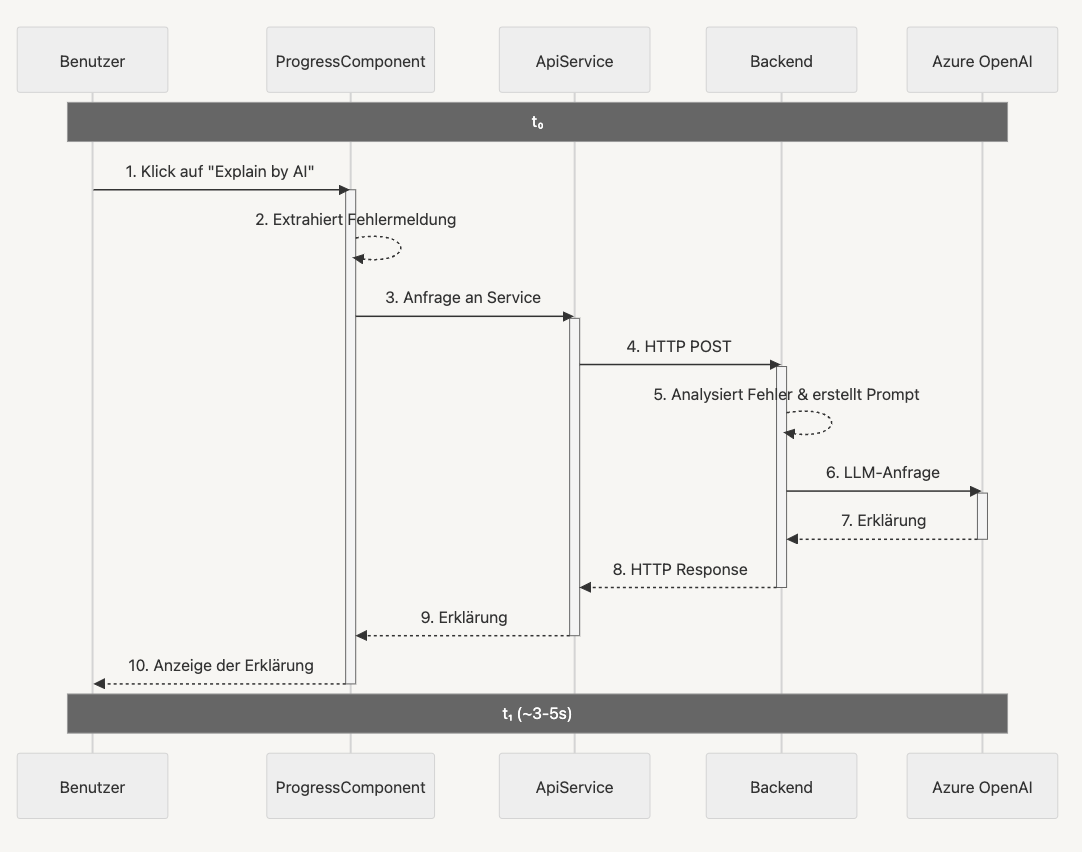
\includegraphics[keepaspectratio]{img/DatenflussSequenzdiagramm.png}}

}

\caption{Datenfluss Sequenzdiagramm}

\end{figure}%

Der detaillierte Datenfluss bei einer typischen Anfrage umfasst acht
Schritte: von der Benutzerinteraktion über die Extraktion der
Fehlermeldung, die HTTP-Anfrage, die Weiterleitung ans Backend, die
Fehleranalyse und Prompt-Erstellung, die LLM-Interaktion bis zur
Rückgabe und Anzeige der Erklärung. Dieser Prozess dauert typischerweise
3-5 Sekunden, was als akzeptable Reaktionszeit eingestuft wurde
(Abbildung 1).

\subsubsection{Entwicklungs- und
Zielumgebung}\label{entwicklungs--und-zielumgebung}

Das CAS-System selbst ist in einem Kubernetes-Cluster deployed, während
CASGPT derzeit als Prototyp in einer lokalen Entwicklungsumgebung läuft.
Die lokale Entwicklung erfolgt mithilfe von Docker-Containern, um die
Portabilität zu gewährleisten und eine konsistente Entwicklungsumgebung
für alle Teammitglieder zu schaffen. Die Fehlermeldungen werden vom
internen Life Cycle Management (LCM) generiert, das für die
Orchestrierung des gesamten Deployment-Prozesses verantwortlich ist. Für
die zukünftige vollständige Integration ist ein Deployment in der
bestehenden Kubernetes-Infrastruktur geplant.

\subsection{Prompt-Engineering und
-Konfiguration}\label{prompt-engineering-und--konfiguration}

\subsubsection{Architektur der
Prompt-Konfiguration}\label{architektur-der-prompt-konfiguration}

Das Prompt-Engineering bildet das Herzstück des CASGPT-Systems und
repräsentiert einen zentralen Feed-Forward-Aspekt der Implementierung.
Die Prompt-Konfiguration ist als eigenständige Komponente
(\texttt{PromptConfig}) implementiert, um eine klare Trennung der
Verantwortlichkeiten zu gewährleisten und zukünftige Erweiterungen im
Sinne des Feed-Forward/Feed-Backward-Paradigmas zu erleichtern (White et
al., 2023). Der detaillierte Workflow des Prompt-Engineering-Prozesses
veranschaulicht die Entwicklung von einer einfachen Erklärung hin zu
einer ursachenabhängigen, mit Kategorien angereicherten und formatierten
Erklärung (Abbildung A.3).

Die Hauptklassen der Implementierung umfassen:

\begin{itemize}
\item
  \textbf{PromptConfig:} Zentrale Klasse für die Initialisierung der
  Konfiguration und die Bereitstellung von Methoden zur Generierung von
  System- und Error-Prompts
\item
  \textbf{ErrorType (Enum):} Definition verschiedener Fehlertypen
  (System Error, User-Fixable Error, etc.)
\item
  \textbf{ErrorCategory:} Repräsentation einer Fehlerkategorie mit
  zugehörigen Mustern, Kontext und Fehlertyp
\item
  \textbf{ErrorPattern:} Definition eines Musters zur Erkennung einer
  Fehlerkategorie mit Gewichtungsfaktor
\item
  \textbf{Message:} Repräsentation einer Nachricht mit Rolle und Inhalt
  für die LLM-Kommunikation
\end{itemize}

\begin{figure}[H]

{\centering \pandocbounded{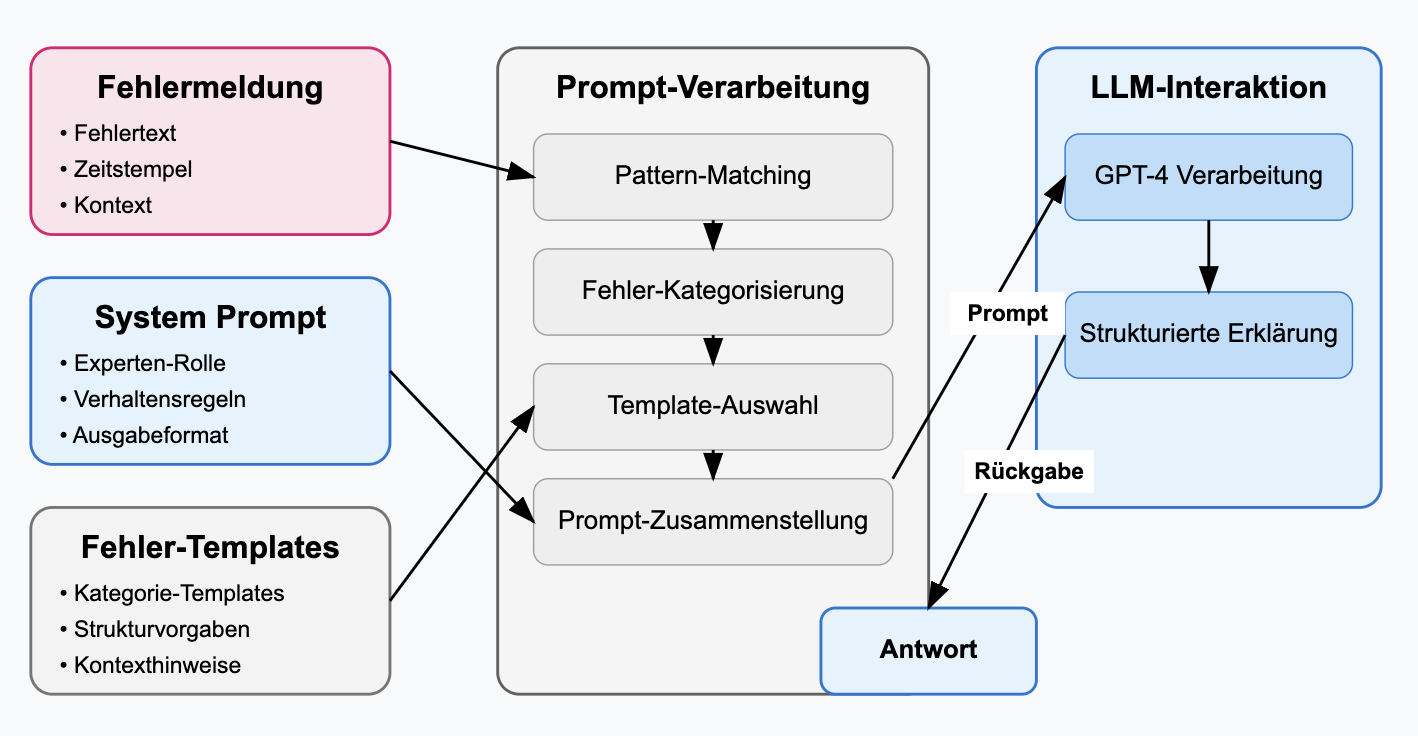
\includegraphics[keepaspectratio]{img/PromptFlowDiagramm.png}}

}

\caption{Prompt Flow Diagramm}

\end{figure}%

Die Fehlerkategorisierung basiert auf einem Mustererkennungssystem mit
regulären Ausdrücken und einem gewichteten Scoring-Mechanismus. Das
System umfasst sieben Hauptkategorien typischer CAS-Fehler:
Datenverarbeitung, Service-Verfügbarkeit, Konfiguration, Deployment,
Netzwerk, Laufzeitausnahmen und eine allgemeine Kategorie. Durch die
Analyse von Log-Dateien mit dem LLM Claude 3.5 Sonnet wurden die
Fehlerkategorien ermittelt. Der Musterabgleich prüft die regulären
Ausdrücke jeder Kategorie gegen die eingehende Fehlermeldung und
berechnet einen Score basierend auf Gewichtung und Spezifität der
Muster. Die Kategorie mit dem höchsten Score wird für die Fehlermeldung
ausgewählt, wodurch eine präzise Kategorisierung und zielgerichtete
Erklärungen ermöglicht werden (Vorobyov et al., 2021; Abbildung A2; Code
A.10).

\subsubsection{Prompt-Struktur}\label{prompt-struktur}

Die Prompt-Struktur orientiert sich an Best Practices und ist in drei
Hauptkomponenten unterteilt:

1. \textbf{System Prompt:}~Dieser Prompt legt die grundlegende Rolle und
das erwartete Verhalten des LLM fest und bleibt über alle Anfragen
hinweg konstant. Er definiert das LLM als Experten für Fehlererklärungen
im Kontext der Deployment-Infrastruktur von CAS.

2. \textbf{Error Prompts:}~Diese Prompts werden dynamisch auf Basis der
identifizierten Fehlerkategorie generiert. Sie enthalten die originale
Fehlermeldung, die zugeordnete Kategorie, relevanten
kategoriespezifischen Kontext und aus der Fehlermeldung extrahierte
Schlüsselwörter.

3. \textbf{Response Templates:}~Diese Templates definieren die erwartete
Struktur der LLM-Antwort. Sie variieren je nach Fehlertyp (z.B.
Standard, Quick-Fix, User-Error), um sicherzustellen, dass die
Erklärungen jeweils die relevantesten Informationen enthalten (Ursache,
Auswirkung, Lösungsschritte).

Das übergeordnete Ziel der Prompt-Gestaltung ist es, technische Konzepte
auch für Benutzer mit unterschiedlichem Vorwissen verständlich zu machen
und Fehlermeldungen in eine möglichst natürliche und zugängliche Sprache
zu übersetzen. Der vollständige System Prompt sowie Beispiele für Error
Prompts und Response Templates sind zur Referenz in Anhang C
dokumentiert (Vatsal \& Dubey, 2024; White et al., 2023; Code A.10).

\subsubsection{Aktuelle Einschränkungen und
Abgrenzung}\label{aktuelle-einschruxe4nkungen-und-abgrenzung}

Die aktuelle Implementierung integriert bewusst keinen dynamischen,
systemspezifischen Kontext in den Prompt-Engineering-Prozess. Diese
Abgrenzung wurde vorgenommen, um den Implementierungsumfang realistisch
zu halten, eine definierte Ausgangsbasis für die Evaluation zu schaffen
und das Potenzial für Weiterentwicklung zu demonstrieren. Konkret fehlen
der aktuellen Implementierung wichtige Kontextinformationen wie
spezifische Konfigurationen der betroffenen Dienste, Versionsdetails der
verwendeten Software und Container, Status abhängiger Komponenten sowie
historische Fehlerinformationen für ähnliche Deployments. Diese
fehlenden Kontextinformationen limitieren die Spezifität und
Handlungsrelevanz der Erklärungen, was in den Experteninterviews als
Hauptverbesserungspotential identifiziert wurde und einen zentralen
Aspekt des evolutionären Weiterentwicklungskonzepts bildet.

\subsection{Entwicklungsprozess}\label{entwicklungsprozess}

Das Feature wurde iterativ entwickelt, wobei Feedback aus internen
Demo-Tests und Diskussionen im Team kontinuierlich in die
Designentscheidungen einfloss. Dieser iterative Prozess spiegelt den
Feed-Forward/Feed-Backward-Ansatz wider: ein initiales Design basierend
auf theoretischen Grundlagen (Feed-Forward) und kontinuierliche
Verbesserung basierend auf frühem Feedback (Feed-Backward). Ein
konkretes Beispiel für diesen iterativen Verbesserungsprozess ist die
Evolution der Prompts von einfachen Anfragen (``Explain this error
message: \{error\_message\}'') zu strukturierten, kontextspezifischen
Prompts mit detaillierten Anweisungen und kategoriespezifischem Kontext
(Abbildung A.3).

\subsection{Technische
Herausforderungen}\label{technische-herausforderungen}

Bei der Implementierung von CASGPT waren zwei zentrale technische
Herausforderungen zu bewältigen:

\textbf{Integration in bestehende Systemkomponenten:} Die nahtlose
Einbindung in die Architektur des CAS-Systems erforderte tiefgreifendes
Verständnis der bestehenden Komponenten und Datenflüsse. Besonders die
Erweiterung der ProgressComponent und des ApiService sowie die
Integration in das Gateway unter Beibehaltung der Sicherheitsmechanismen
stellten anspruchsvolle Aufgaben dar.

\textbf{Prompt-Konfiguration:} Die Entwicklung eines effektiven
Kategorisierungssystems mit Mustern für verschiedene Fehlertypen
erforderte umfangreiche Analyse realer Fehlermeldungen. Die größte
Herausforderung bestand darin, eine Balance zwischen generalisierten
Erklärungen für diverse Fehler und spezifischen, handlungsrelevanten
Informationen zu finden. Der iterative Ansatz zur Verfeinerung der
Prompt-Konfiguration anhand von Testfällen mit realen Fehlermeldungen
ermöglichte die schrittweise Optimierung der Erklärungsqualität.

\subsection{Sicherheitsaspekte}\label{sicherheitsaspekte}

\subsubsection{Sicherheitsmaßnahmen}\label{sicherheitsmauxdfnahmen}

Bei der Implementierung wurden verschiedene Sicherheitsmaßnahmen
getroffen, um den Enterprise-Anforderungen gerecht zu werden:

1. Nutzung eines intern gehosteten LLM in Schweden für Datensouveränität
und DSGVO-Konformität

2. direkte Extraktion der Fehlermeldungen aus Systemlogs zur Vermeidung
von XSS-Schwachstellen

3. Integration in bestehende Sicherheitsmechanismen des API-Gateways

4. sichere Speicherung sensitiver Tokens in Vault.

Diese Maßnahmen stellen sicher, dass CASGPT keine neuen
Sicherheitsrisiken einführt.

\subsubsection{Umgang mit
LLM-Limitationen}\label{umgang-mit-llm-limitationen}

CASGPT implementiert mehrere gezielte Maßnahmen, um den diskutierten
Limitationen zu begegnen:

\textbf{Gegen Halluzinationen:} - Strukturierte Prompts mit klaren
Antwortformaten

\begin{itemize}
\item
  Reflection Pattern zur kritischen Selbstreflexion des LLM
\item
  Template Pattern zur Strukturierung der Ausgaben
\end{itemize}

\textbf{Gegen mangelndes Systemkontextwissen:}

\begin{itemize}
\item
  Fehlerkategorisierung für kategoriespezifischen Kontext
\item
  Kontextuelle Anreicherung durch Extraktion relevanter Informationen
\item
  Bewusste Abgrenzung zur Schaffung einer definierten Evaluationsbasis
\end{itemize}

Diese Gegenmaßnahmen bilden die Grundlage für die initiale
Implementierung und werden im Rahmen der evolutionären Weiterentwicklung
optimiert.

\section{Evaluation und Analyse}\label{evaluation-und-analyse}

\subsection{Methodik der Evaluation}\label{methodik-der-evaluation}

Die Evaluation des CASGPT-Systems erfolgte mittels halbstrukturierter
Experteninterviews mit drei Schlüsselpersonen: einem Product Owner (P),
einem Full-Stack-Entwickler (M) und einem DevOps Engineer (D). Diese
multiperspektivische Herangehensweise ermöglicht eine ganzheitliche
Beurteilung des Systems (Engström et al., 2020).

Die etwa 45-60-minütigen Interviews wurden protokolliert und mittels
qualitativer Inhaltsanalyse ausgewertet (Mayring, 2014; Notizen A.12)).
Die Analyse erfolgte durch ein kombiniert deduktiv-induktives
Kodierungsverfahren, wobei zunächst theoriegeleitete Hauptkategorien
definiert und anschließend induktiv weitere Kategorien aus dem Material
entwickelt wurden.

\subsection{Zentrale
Evaluationsergebnisse}\label{zentrale-evaluationsergebnisse}

Die qualitative Analyse der Interviews ergab mehrere zentrale
Erkenntnisse:

Der \textbf{Bedarf an systemspezifischem Kontext} wurde am häufigsten
thematisiert (8 Nennungen), gefolgt vom \textbf{Mangel an Spezifität} in
den Erklärungen (6 Nennungen) und dem wahrgenommenen \textbf{Potenzial
des Systems} (6 Nennungen). Der \textbf{Beitrag zum Benutzerverständnis}
wurde ebenfalls als wesentlicher positiver Aspekt hervorgehoben (5
Nennungen).

Diese quantitative Verteilung deutet auf ein grundsätzlich wertvolles
System hin, das durch die Integration von spezifischem Systemwissen
deutlich verbessert werden könnte (Tabelle A.8).

\subsection{Thematische Analyse und rollenspezifische
Perspektiven}\label{thematische-analyse-und-rollenspezifische-perspektiven}

\subsubsection{Systemkontext als
Hauptlimitation}\label{systemkontext-als-hauptlimitation}

Alle drei Experten identifizierten den mangelnden Systemkontext als
zentrale Einschränkung:

\begin{quote}
``Ja, die System Knowledge fehlt, die man in die Prompts einbauen
sollte'' (D)

``Wenn System Knowledge (Wiki Dump) dem Model gegeben wird, hat es mehr
Ahnung worum es geht'' (M)
\end{quote}

Der DevOps Engineer betonte den Bedarf an spezifischeren
Handlungsempfehlungen, während der Full-Stack-Entwickler auf die
technische Umsetzbarkeit durch Integration von Systemdokumentation
fokussierte. Der Product Owner sah dies als Möglichkeit zur Erhöhung des
Systemwerts.

\subsubsection{Grundnutzen und
Transparenz}\label{grundnutzen-und-transparenz}

Trotz der identifizierten Einschränkungen bestätigten alle Interviews
den Mehrwert des Systems:

\begin{quote}
``Doch schon einiges an Hilfe, nicht jeder User weiß, was ein DSO ist''
(M)

``Wertschöpfung: für Menschen komisch wirkenden Fehler in natürliche
Sprache übersetzen'' (P)
\end{quote}

Der Hauptwert liegt in der Übersetzungsleistung von technischen Details
in verständliche Sprache und der damit verbundenen Transparenz und
Vertrauensbildung.

\subsubsection{Integration und
Akzeptanz}\label{integration-und-akzeptanz}

Die Integration des Features in den bestehenden Workflow wurde
einheitlich positiv bewertet, wobei die nahtlose Implementierung in die
Benutzeroberfläche und die Übereinstimmung mit den Nutzererwartungen
hervorgehoben wurden. Der DevOps Engineer identifizierte die Antwortzeit
als kritischen Faktor: ``Nicht zu hohe Latenz zwischen der
Antwort\ldots{} wenn man so ca. 5 Sekunden wartet ist's okay'' (D).

\subsubsection{Entwicklungspotenzial}\label{entwicklungspotenzial}

Als konkrete Erweiterungsmöglichkeiten wurden vorgeschlagen:

\begin{itemize}
\tightlist
\item
  \textbf{BlueBox-übergreifender Wissenstransfer}: ``Wenn Fehler bei
  einer anderen BlueBox war, direkt in Prompt mit schreiben - das war
  übrigens der Fix'' (D)
\item
  \textbf{Interaktives Chatfenster}: ``Weiterentwicklung: interaktiver:
  z.B. in die Erklärung ein Chatfenster → KI nochmal Nachfragen
  stellen'' (P)
\item
  \textbf{Feedbackmechanismen}: ``Selbstlernend immer sinnvoll →
  Antwortqualität bewerten'' (M)
\end{itemize}

\section{Evolutionäres
Weiterentwicklungskonzept}\label{evolutionuxe4res-weiterentwicklungskonzept}

\subsection{Zielzustand und
Wertbeitrag}\label{zielzustand-und-wertbeitrag}

Der angestrebte Zielzustand entwickelt das aktuelle CASGPT von
generischen Erklärungen (Wang et al., 2023) zu spezifischen,
kontextbewussten Erklärungen; von statischer Prompt-Konfiguration zu
kontinuierlicher, feedback-basierter Verbesserung (Ouyang et al., 2022);
von reaktiver zu proaktiver, vorhersagebasierter Fehlerbehandlung (Ahmed
et al., 2023); von einmaliger Erklärung zu dialogbasierter Interaktion
(Wu et al., 2022); und von keiner Lernfähigkeit zu systematischem
Feedback-basiertem Lernen (Li et al., 2021). Ein detaillierter Vergleich
zwischen dem aktuellen Zustand und dem Zielzustand wurde erarbeitet
(Tabelle A.9).

Dieser Zielzustand verspricht mehrere konkrete Wertbeiträge:

1. \textbf{Erhöhte Benutzerproduktivität} durch präzisere,
kontextspezifische Erklärungen

2. \textbf{Reduzierter Supportaufwand} durch verbesserte
Selbsthilfe-Möglichkeiten

3. \textbf{Verbesserte Systemzuverlässigkeit} durch proaktive
Fehlervermeidung

4. \textbf{Kontinuierliche Wissenserweiterung} als selbstverstärkender
Lernprozess

Dieser Zielstand orientiert sich an dem Rahmen des
Feed-Forward/Feed-Backward-Ansatzes, der die gesamte CASGPT-Entwicklung
charakterisiert.

\subsection{Feed-Forward/Feed-Backward-Integration}\label{feed-forwardfeed-backward-integration}

\subsubsection{MAPE-K-Schleife als strukturelles
Rahmenwerk}\label{mape-k-schleife-als-strukturelles-rahmenwerk}

Um den Feed-Forward/Feed-Backward-Ansatz in ein operatives Designprinzip
zu überführen, wird das MAPE-K-Framework (Monitor, Analyze, Plan,
Execute, Knowledge) für selbstadaptive Systeme (Cheng et al., 2009) als
strukturelles Rahmenwerk verwendet. Dieses Framework implementiert einen
geschlossenen Regelkreis für kontinuierliches Lernen und integriert
Feedback-Mechanismen in einen strukturierten Adaptionsprozess:

\begin{itemize}
\item
  \textbf{Monitor:} Sammlung von Fehlermeldungen, Benutzerfeedback und
  Systemmetriken
\item
  \textbf{Analyze:} Musteranalyse, Fehlerkategorisierung und
  Feedbackauswertung
\item
  \textbf{Plan:} Optimierung der Prompts und Erweiterung der
  Wissensbasis
\item
  \textbf{Execute:} Anwendung optimierter Prompts und Integration neuen
  Wissens
\item
  \textbf{Knowledge:} Zentrale Wissensbasis mit Systemkontext und
  Fehlermustern
\end{itemize}

Der Knowledge-Bereich dient dabei als gemeinsame Grundlage für
Feed-Forward (Anwendung von Wissen) und Feed-Backward (Integration neuen
Wissens).

\subsubsection{Feedback-Mechanismen als
Kernelemente}\label{feedback-mechanismen-als-kernelemente}

Basierend auf den Experteninterviews (M: ``selbstlernend immer sinnvoll
→ Antwortsqualität bewerten'') werden folgende Feedback-Mechanismen
konzipiert:

\textbf{1. Explizites Feedback:}

\begin{itemize}
\item
  \textbf{Qualitätsbewertung:} Einfaches Bewertungssystem (+/-) nach
  jeder Erklärung
\item
  \textbf{Kategorisiertes Feedback:} Vorgegebene Kategorien wie ``Zu
  technisch'', ``Zu vage''
\item
  \textbf{Verbesserungsvorschläge:} Freitextfeld für konkrete Anregungen
\end{itemize}

\textbf{2. Implizites Feedback:}

\begin{itemize}
\item
  \textbf{Wiederkehrende Fehler:} Automatische Erkennung von Fällen, in
  denen derselbe Fehler nach einer Erklärung erneut auftritt
\item
  \textbf{Nutzungsstatistiken:} Analyse der Nutzungsmuster (z.B.
  Häufigkeit der Feature-Nutzung)
\end{itemize}

\subsubsection{BlueBox-übergreifender
Wissenstransfer}\label{bluebox-uxfcbergreifender-wissenstransfer}

Ein besonders effektiver Mechanismus zur Systemverbesserung ist die
Übertragung von Lösungen zwischen verschiedenen BlueBoxes, wie vom
DevOps Engineer hervorgehoben:

\begin{quote}
``Wenn Fehler bei einer anderen BlueBox war, direkt in Prompt mit
schreiben - das war übrigens der Fix → BlueBox kann das selber machen
{[}\ldots{]} Spart Zeit → weniger Supportaufwand bei selbem Fehler'' (D)
\end{quote}

Dieser Ansatz implementiert einen selbstverstärkenden Lernmechanismus
durch:

1. \textbf{Erfassung erfolgreicher Fixes:} Dokumentation erfolgreicher
Fehlerbehebungen mit Kontext

2. \textbf{Erkennung ähnlicher Fehler:} Automatische Identifikation von
Ähnlichkeiten zu früheren Fehlern

3. \textbf{Integration von Lösungswissen:} Wiederverwendung bewährter
Lösungsansätze in neuen Kontexten

\subsection{Systematische Analyse für proaktive
Fehlervorhersage}\label{systematische-analyse-fuxfcr-proaktive-fehlervorhersage}

\subsubsection{Clustering von
Fehlermeldungen}\label{clustering-von-fehlermeldungen}

Zur Identifikation ähnlicher Fehler wird ein Clustering-Ansatz
implementiert, der die Grundlage für den BlueBox-übergreifenden
Wissenstransfer bildet (Vorobyov et al., 2021):

\begin{itemize}
\item
  \textbf{Aufbereitung der Fehlertexte:} Entfernung variabler Elemente
  wie Zeitstempel und Tokenisierung
\item
  \textbf{Gruppierung:} Anwendung von k-Means oder DBSCAN zur
  automatischen Cluster-Bildung
\item
  \textbf{Anwendung für Prompt-Optimierung:} Entwicklung spezifischer
  Prompt-Templates für häufige Fehlerklassen
\end{itemize}

Das Clustering ermöglicht eine klarere Unterscheidung zwischen
nutzerseitigen und systemseitigen Fehlern -- ein Aspekt, der in den
Interviews als wichtig hervorgehoben wurde.

\subsubsection{Association Rule Mining für
Fehlervorhersage}\label{association-rule-mining-fuxfcr-fehlervorhersage}

Association Rule Mining (ARM) dient zur Identifikation von
Zusammenhängen zwischen Konfigurationsparametern und Fehlertypen (Wang
et al., 2022; Li et al., 2024):

\begin{itemize}
\item
  \textbf{Regelextraktion:} Anwendung von Algorithmen wie Apriori oder
  FP-Growth
\item
  \textbf{Praktische Anwendung:} Übersetzung der Regeln in verständliche
  Warnungen und Empfehlungen
\end{itemize}

Durch die Kombination von Clustering und ARM können Fehlermuster
systematisch identifiziert und für die Verbesserung des Systems genutzt
werden, was direkt auf die zweite Unterforschungsfrage einzahlt.

\textbf{Beispiel für Assoziationsregeln:}

\begin{quote}
\texttt{WENN\ (service\_version="1.2.3"\ UND\ network\_config="internal")\ DANN\ Wahrscheinlichkeit\ für\ Fehlertyp\ "permission\_denied"\ =\ 78\%\ EMPFEHLUNG:\ "Überprüfen\ Sie\ die\ Berechtigungen\ vor\ dem\ Deployment"}
\end{quote}

\subsection{Proaktive Fähigkeiten}\label{proaktive-fuxe4higkeiten}

\subsubsection{Kontextsensitive
Erklärungen}\label{kontextsensitive-erkluxe4rungen}

Die Integration von Systemkontext in die Erklärungen bildet die
Grundlage für proaktive Fähigkeiten. Durch die dynamische Einbindung von
Konfigurationsinformationen, Systemarchitektur und Abhängigkeiten können
Erklärungen deutlich spezifischer und handlungsrelevanter gestaltet
werden. Dies umfasst die: Automatische Extraktion relevanter
Konfigurationsparameter, Integration von Systemarchitekturwissen und
Berücksichtigung von Service-Interaktionen und Abhängigkeiten.

\subsubsection{Interaktive
Fehleranalyse}\label{interaktive-fehleranalyse}

Entsprechend dem Vorschlag des Product Owners zur Erweiterung des
Systems um interaktive Funktionen: \textgreater{} ``Weiterentwicklung:
interaktiver: z.B. in die Erklärung ein Chatfenster → KI nochmal
Nachfragen stellen'' (P)

Das System kann um einen dialogorientierten Ansatz erweitert werden, bei
dem Benutzer Rückfragen zu Erklärungen stellen können. Dies unterstützt
den Übergang zu einem proaktiveren System durch:

\begin{itemize}
\item
  \textbf{Vertiefende Erklärungen:} Detailliertere Informationen zu
  spezifischen Aspekten eines Fehlers
\item
  \textbf{Schrittweise Fehleranalyse:} Geführte Exploration der
  Fehlerursachen
\item
  \textbf{Kontextualisierte Lösungsvorschläge:} Anpassung der
  Lösungsvorschläge an die spezifische Situation des Benutzers
\end{itemize}

\subsection{Technische Verbesserungen und
Priorisierung}\label{technische-verbesserungen-und-priorisierung}

Die Evolution zu einem selbstlernenden System erfordert zusätzliche
Komponenten und eine priorisierte Umsetzung. Basierend auf den
Experteninterviews, der technischen Machbarkeit und dem erwarteten
Wertbeitrag wird folgende Implementierungsstrategie vorgeschlagen:

\textbf{Hohe Priorität:}

\begin{itemize}
\item
  Systemkontext-Integration: Implementierung eines
  Systemkontext-Connectors zur dynamischen Einbindung von
  CAS-Komponenten und Konfigurationsinformationen
\item
  Einfacher Feedback-Mechanismus: Einführung eines ``Hilfreich/Nicht
  hilfreich''-Buttons mit Feedback-Datenbank zur Bewertungsspeicherung
\item
  BlueBox-übergreifender Wissenstransfer: Entwicklung von Mechanismen
  zur Dokumentation und Wiederverwendung erfolgreicher Fehlerbehebungen
\end{itemize}

\textbf{Mittlere Priorität:}

\begin{itemize}
\item
  Verbesserte Fehlerkategorisierung und Cluster-Erkennung mittels
  Analyse-Engine
\item
  Konfigurationsempfehlungen basierend auf historischen Daten
\item
  Erweiterter Prompt-Generator mit interaktiver Chatbot-Funktionalität
\end{itemize}

Diese inkrementelle Umsetzungsstrategie gewährleistet, dass jede
Implementierungsphase einen konkreten Mehrwert liefert und gleichzeitig
die Grundlage für nachfolgende Erweiterungen schafft.

\section{Fazit}\label{fazit}

\subsection{Zusammenfassung der
Forschungsergebnisse}\label{zusammenfassung-der-forschungsergebnisse}

Diese Arbeit untersuchte die Evolution eines LLM-basierten
Fehlererklärungssystems zu einem selbstlernenden System durch
systematische Analyse und Feedback. Durch den
Feed-Forward/Feed-Backward-Ansatz wurden theoretische Grundlagen,
praktische Implementierung und ein evolutionäres
Weiterentwicklungskonzept erarbeitet.

Die zentralen Ergebnisse sind:

\begin{enumerate}
\def\labelenumi{\arabic{enumi}.}
\tightlist
\item
  \textbf{Erfolgreiche LLM-Integration:} Die CASGPT-Implementierung
  demonstriert die effektive Nutzung von LLMs zur Verbesserung der
  Benutzererfahrung bei komplexen Cloud-Deployments (Brown et al., 2020;
  Wang et al., 2023).
\item
  \textbf{Systemkontext als kritische Limitierung:} Die Evaluation
  identifizierte mangelnden Systemkontext als zentrale Einschränkung,
  was die Notwendigkeit einer dynamischen Kontextintegration
  unterstreicht (Talukdar \& Biswas, 2023).
\item
  \textbf{MAPE-K als Evolutionsrahmen:} Das MAPE-K-Framework bietet ein
  strukturiertes Modell für die Evolution zu einem selbstlernenden
  System (Cheng et al., 2009; Wong et al., 2022).
\item
  \textbf{Proaktive Fähigkeiten als Ziel:} Der konzipierte Übergang von
  reaktiven Erklärungen zu proaktiven Empfehlungen und Fehlervorhersagen
  zeigt das Potenzial der Kombination von LLMs mit
  Mustererkennungstechniken (Vorobyov et al., 2021; Wang et al., 2022).
\end{enumerate}

Diese Ergebnisse adressieren direkt die Hauptforschungsfrage zur
Evolution eines LLM-basierten Fehlererklärungssystems zu einem
selbstlernenden System und liefern konkrete Konzepte für die praktische
Umsetzung.

\subsection{Praktische Implikationen}\label{praktische-implikationen}

Die Forschungsergebnisse haben wichtige praktische Implikationen für
Organisationen:

\begin{itemize}
\tightlist
\item
  Bereits ein Basissystem ohne umfassenden Systemkontext bietet durch
  verbesserte Transparenz einen Mehrwert für Benutzer und
  Organisationen. Die Experteninterviews bestätigten, dass selbst
  generische Erklärungen zu einem besseren Verständnis komplexer
  Fehlermeldungen beitragen können.
\item
  Die schrittweise Evolution ermöglicht einen inkrementellen Ansatz mit
  kontinuierlichem Wertbeitrag. Organisationen können mit grundlegenden
  Funktionen beginnen und das System systematisch erweitern, ohne
  umfangreiche Vorabinvestitionen.
\item
  Feedback ist die Schlüsselressource für den Übergang zu
  selbstlernenden Systemen. Die konsequente Sammlung und Analyse von
  Benutzerfeedback bildet die Grundlage für kontinuierliche Verbesserung
  und Adaptation.
\end{itemize}

Diese Implikationen gelten nicht nur für Fehlererklärungssysteme,
sondern können auf weitere KI-gestützte Assistenzsysteme in
Enterprise-Umgebungen übertragen werden (Devaraju, 2024; Perron et al.,
2025).

\subsection{Limitationen und kritische
Reflexion}\label{limitationen-und-kritische-reflexion}

Diese Arbeit unterliegt mehreren Limitationen:

\begin{itemize}
\tightlist
\item
  \textbf{Prototypischer Charakter:} Das volle Potenzial des Systems
  würde sich erst im langfristigen produktiven Einsatz zeigen. Die
  tatsächliche Nutzungserfahrung könnte zu weiteren Erkenntnissen
  führen, die im Rahmen dieser Arbeit nicht antizipiert werden konnten.
\item
  \textbf{Konzeptionelle vs.~implementierte Evolution:} Das
  Weiterentwicklungskonzept wurde theoretisch ausgearbeitet, aber nicht
  vollständig implementiert. Die praktische Umsetzung könnte zusätzliche
  Herausforderungen offenbaren, die weitere Anpassungen erfordern.
\item
  \textbf{Generalisierbarkeit:} Die Ergebnisse beziehen sich spezifisch
  auf den CAS-Kontext und Deployment-Fehler im Cloud-Umfeld. Obwohl die
  grundlegenden Prinzipien übertragbar sein dürften, können in anderen
  Domänen spezifische Anpassungen erforderlich sein.
\end{itemize}

\subsection{Ausblick}\label{ausblick}

Diese Forschung eröffnet mehrere vielversprechende Richtungen für
zukünftige Arbeit:

\begin{itemize}
\tightlist
\item
  \textbf{Erweiterte Lernmethoden:} Integration von Reinforcement
  Learning from Human Feedback (RLHF) (Stiennon et al., 2020) und
  ausgereifteren Human-in-the-Loop-Ansätzen (Wu et al., 2022). Diese
  könnten die Adaptivität des Systems weiter verbessern und den Übergang
  zu einem vollständig selbstlernenden System beschleunigen.
\item
  \textbf{Multi-Agent-Systeme:} Verteilte Fehleranalyse durch
  spezialisierte Agenten für verschiedene Aspekte der Systemdiagnose.
  Dieses Konzept könnte die Skalierbarkeit und Spezifität der
  Fehleranalyse verbessern, indem verschiedene Agenten für
  unterschiedliche Systemkomponenten oder Fehlertypen spezialisiert
  werden.
\item
  \textbf{Domänenadaption:} Übertragung des Konzepts auf andere
  Cloud-Plattformen und Deployment-Umgebungen. Die generischen
  Prinzipien des Feed-Forward/Feed-Backward-Ansatzes und der
  systematischen Evolution könnten auf andere technische Domänen
  angewendet werden.
\item
  \textbf{Balance zwischen Erklärbarkeit und Leistungsfähigkeit:}
  Weitere Forschung zur optimalen Balance zwischen detaillierten,
  transparenten Erklärungen und effizienter, prägnanter Kommunikation
  ist notwendig. Dies betrifft insbesondere die Frage, wie viel Kontext
  und technisches Detail für verschiedene Benutzergruppen hilfreich ist.
\item
  \textbf{Vertrauen in KI-generierte Erklärungen:} Untersuchung der
  Faktoren, die das Vertrauen in LLM-generierte technische Erklärungen
  beeinflussen. Die Akzeptanz solcher Systeme hängt maßgeblich vom
  Vertrauen der Benutzer ab, was weitere Forschung zu Transparenz,
  Konsistenz und Nachvollziehbarkeit erfordert.
\end{itemize}

Die Evolution von LLM-basierten Assistenzsystemen steht noch am Anfang.
Diese Arbeit liefert einen Beitrag durch die systematische Untersuchung
der Integration und Evolution eines spezifischen Anwendungsfalls, bietet
jedoch gleichzeitig einen konzeptionellen Rahmen für die weitere
Erforschung selbstlernender KI-Systeme in Enterprise-Umgebungen.

\appendix
\renewcommand{\thefigure}{A\arabic{figure}}
\renewcommand{\thetable}{A\arabic{table}}
\setcounter{figure}{0}
\setcounter{table}{0}

\section{Anhang}\label{anhang}

\subsection{User Interface}\label{user-interface}

\pandocbounded{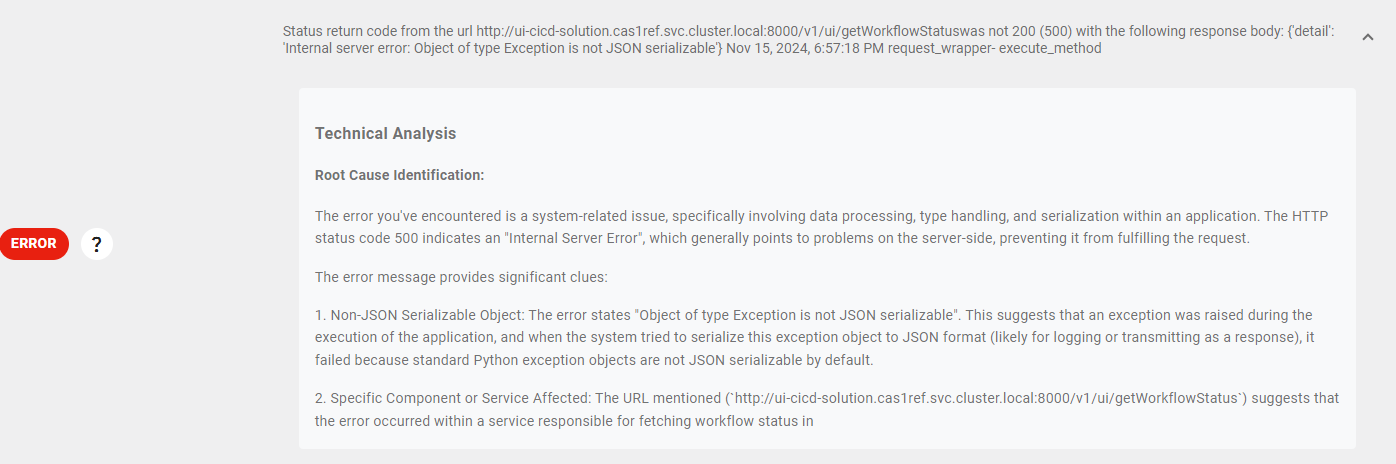
\includegraphics[keepaspectratio]{img/JSON.png}}

\newpage

\subsection{detailliertes Komponenten
Diagramm}\label{detailliertes-komponenten-diagramm}

\pandocbounded{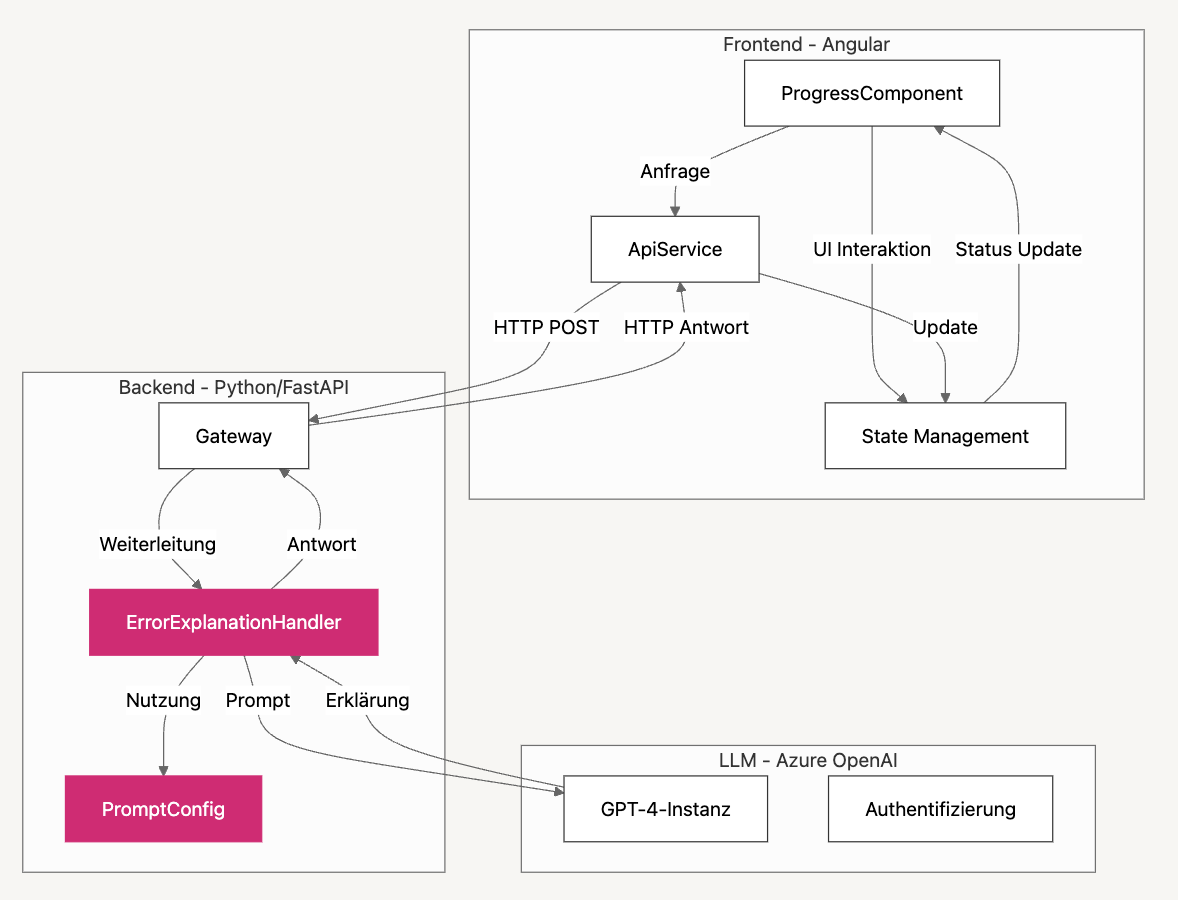
\includegraphics[keepaspectratio]{img/KomponentenDiagrammDetailliert.png}}

\newpage

\subsection{Prompt-Engineering
Workflow}\label{prompt-engineering-workflow}

\pandocbounded{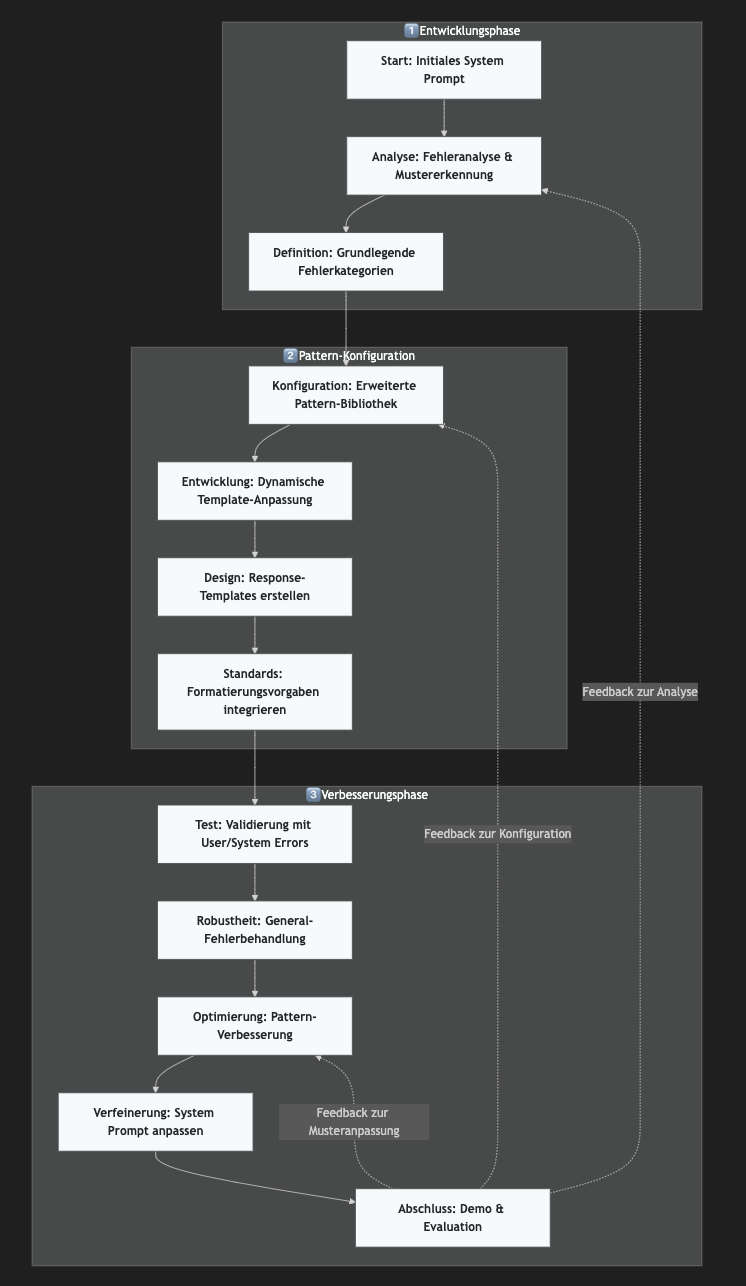
\includegraphics[keepaspectratio]{img/PromptEngineeringWorkflow.png}}

\newpage

\subsection{Chancen und Herausforderungen bei der Integration von LLMs
in
Enterprise-Systemen}\label{chancen-und-herausforderungen-bei-der-integration-von-llms-in-enterprise-systemen}

\begin{longtable}[]{@{}
  >{\raggedright\arraybackslash}p{(\linewidth - 4\tabcolsep) * \real{0.1600}}
  >{\raggedright\arraybackslash}p{(\linewidth - 4\tabcolsep) * \real{0.3500}}
  >{\raggedright\arraybackslash}p{(\linewidth - 4\tabcolsep) * \real{0.4850}}@{}}
\toprule\noalign{}
\begin{minipage}[b]{\linewidth}\raggedright
\textbf{Chancen}
\end{minipage} & \begin{minipage}[b]{\linewidth}\raggedright
\textbf{Beschreibung}
\end{minipage} & \begin{minipage}[b]{\linewidth}\raggedright
\textbf{Herausforderungen:}

\textbf{Beschreibung}
\end{minipage} \\
\midrule\noalign{}
\endhead
\bottomrule\noalign{}
\endlastfoot
\begin{minipage}[t]{\linewidth}\raggedright
Automati-\\
sierung\strut
\end{minipage} & Reduktion manueller Prozesse durch natürlichsprachliche
Interaktion & \textbf{Sicherheit}: Schutz sensibler Daten und
Konformität mit Zero-Trust-Architektur (Dash, 2024) \\
Verbesserte Benutzererfahrung & Vereinfachung komplexer technischer
Inhalte & \textbf{Ressourcenbedarf}: Hohe Anforderungen an
Rechenleistung und Speicher (Hu et al., 2021) \\
Wissens-

distribution & Demokratisierung von Expertenwissen & \textbf{Datenschutz
\& Compliance}: Einhaltung von Regularien wie DSGVO (Devaraju, 2024) \\
Integrations-

fähigkeit & Brückentechnologie zwischen verschiedenen Systemen &
\textbf{Interpretierbarkeit}: Nachvollziehbarkeit von Entscheidungen
(Kumar et al., 2025) \\
Skalier-

barkeit & Bewältigung wachsender und diverser Fehlertypen &
\textbf{Wartbarkeit}: Kontinuierliche Anpassung und Optimierung
(Alibakhsh, 2023) \\
\end{longtable}

\newpage

\subsection{Vergleich verschiedener
Fehlererklärungsansätze}\label{vergleich-verschiedener-fehlererkluxe4rungsansuxe4tze}

\begin{longtable}[]{@{}
  >{\raggedright\arraybackslash}p{(\linewidth - 8\tabcolsep) * \real{0.2121}}
  >{\raggedright\arraybackslash}p{(\linewidth - 8\tabcolsep) * \real{0.2424}}
  >{\raggedright\arraybackslash}p{(\linewidth - 8\tabcolsep) * \real{0.1030}}
  >{\raggedright\arraybackslash}p{(\linewidth - 8\tabcolsep) * \real{0.2545}}
  >{\raggedright\arraybackslash}p{(\linewidth - 8\tabcolsep) * \real{0.1697}}@{}}
\toprule\noalign{}
\begin{minipage}[b]{\linewidth}\raggedright
\textbf{Ansatz}
\end{minipage} & \begin{minipage}[b]{\linewidth}\raggedright
\textbf{Beschreibung}
\end{minipage} & \begin{minipage}[b]{\linewidth}\raggedright
\textbf{Stärken}
\end{minipage} & \begin{minipage}[b]{\linewidth}\raggedright
\textbf{Schwächen}
\end{minipage} & \begin{minipage}[b]{\linewidth}\raggedright
\textbf{Relevanz für CASGPT}
\end{minipage} \\
\midrule\noalign{}
\endhead
\bottomrule\noalign{}
\endlastfoot
\textbf{Traditionelle Ansätze} & & & & \\
Statische Fehlercodes & Standardisierte Fehlermeldungen &
\begin{minipage}[t]{\linewidth}\raggedright
Konsis-\\
tenz\strut
\end{minipage} & Kontextlosigkeit, schwer verständlich & Baseline für
Verbesserung \\
\begin{minipage}[t]{\linewidth}\raggedright
Dokumen-\\
tationen\strut
\end{minipage} & Umfassende Fehlerbeschreibungen & Detailtiefe &
\begin{minipage}[t]{\linewidth}\raggedright
Wartungs-\\
aufwand,\\
Veraltung\strut
\end{minipage} & Ergänzende Wissensquelle \\
Rule-Based Error Handling & Regelbasierte Fehlerbehandlung &
\begin{minipage}[t]{\linewidth}\raggedright
Präzision bei\\
bekannten\\
Fehlern\strut
\end{minipage} & Schlechte Skalierbarkeit & Ergänzender Ansatz \\
\textbf{KI-basierte Ansätze} & & & & \\
Case-Based Reasoning & Lösung basierend auf ähnlichen Fällen &
\begin{minipage}[t]{\linewidth}\raggedright
Praxis-\\
bewährte\\
Lösungen\strut
\end{minipage} & Abhängigkeit von Fallbasis & Konzeptuelle
Ähnlichkeit \\
ML-Clustering & Musterbasierte Fehlerkategorisierung &
\begin{minipage}[t]{\linewidth}\raggedright
Automa-\\
tische\\
Gruppie-\\
rung\strut
\end{minipage} & Keine natürlichsprachlichen Erklärungen & Ergänzende
Technik \\
LLM-basierte Root Cause Analysis & LLM-gestützte Ursachenanalyse &
\begin{minipage}[t]{\linewidth}\raggedright
Natürlich-\\
sprachliche\\
Erklärungen,\\
Adaptivität\strut
\end{minipage} & Halluzinationen, Ressourcenbedarf & Direktes Vorbild \\
\end{longtable}

\newpage

\subsection{Relevante Prompt-Patterns für
Fehlererklärungen}\label{relevante-prompt-patterns-fuxfcr-fehlererkluxe4rungen}

\begin{longtable}[]{@{}
  >{\raggedright\arraybackslash}p{(\linewidth - 4\tabcolsep) * \real{0.1477}}
  >{\raggedright\arraybackslash}p{(\linewidth - 4\tabcolsep) * \real{0.3557}}
  >{\raggedright\arraybackslash}p{(\linewidth - 4\tabcolsep) * \real{0.4899}}@{}}
\toprule\noalign{}
\begin{minipage}[b]{\linewidth}\raggedright
\textbf{Pattern}
\end{minipage} & \begin{minipage}[b]{\linewidth}\raggedright
\textbf{Beschreibung}
\end{minipage} & \begin{minipage}[b]{\linewidth}\raggedright
\textbf{Anwendung in CASGPT}
\end{minipage} \\
\midrule\noalign{}
\endhead
\bottomrule\noalign{}
\endlastfoot
Persona Pattern & Definition einer spezifischen Rolle für das LLM & ``Du
bist ein Experte für Fehlererklärung in Cloud-Deployment-Systemen'' \\
Template Pattern & Vorgabe einer spezifischen Ausgabestruktur &
Strukturierung der Erklärung in Ursache, Auswirkung, Lösung \\
Context Enhancement & Anreicherung mit domänenspezifischem Wissen &
Integration von Systemwissen über CAS-Komponenten \\
Cognitive Verifier & Aufforderung zur Verifizierung der eigenen Antwort
& Selbstprüfung zur Reduktion von Halluzinationen \\
Reflection Pattern & Explizite Aufforderung zur Selbstreflexion &
Erkennung von Unsicherheiten in der Erklärung \\
Chain-of-Thought & Aufforderung zu schrittweisem Denken & Verbesserung
der Reasoning-Fähigkeiten des LLM \\
\end{longtable}

\newpage

\subsection{Kernkonzepte selbstlernender Systeme für
CASGPT}\label{kernkonzepte-selbstlernender-systeme-fuxfcr-casgpt}

\begin{longtable}[]{@{}
  >{\raggedright\arraybackslash}p{(\linewidth - 6\tabcolsep) * \real{0.1258}}
  >{\raggedright\arraybackslash}p{(\linewidth - 6\tabcolsep) * \real{0.4214}}
  >{\raggedright\arraybackslash}p{(\linewidth - 6\tabcolsep) * \real{0.1698}}
  >{\raggedright\arraybackslash}p{(\linewidth - 6\tabcolsep) * \real{0.2704}}@{}}
\toprule\noalign{}
\begin{minipage}[b]{\linewidth}\raggedright
\textbf{Konzept}
\end{minipage} & \begin{minipage}[b]{\linewidth}\raggedright
\textbf{Beschreibung}
\end{minipage} & \begin{minipage}[b]{\linewidth}\raggedright
\textbf{Relevanz für CASGPT}
\end{minipage} & \begin{minipage}[b]{\linewidth}\raggedright
\textbf{Literatur}
\end{minipage} \\
\midrule\noalign{}
\endhead
\bottomrule\noalign{}
\endlastfoot
MAPE-K Loop & Monitor-Analyze-Plan-Execute-Knowledge-Zyklus für
Selbstadaption & \begin{minipage}[t]{\linewidth}\raggedright
Strukturiertes\\
Framework\\
für den Feed-Forward/\\
Feed-Backward-\\
Kreislauf\strut
\end{minipage} & Cheng et al.~(2009) \\
\begin{minipage}[t]{\linewidth}\raggedright
Feedback-\\
Schleifen\strut
\end{minipage} & Systematische Rückkopplungsmechanismen &
\begin{minipage}[t]{\linewidth}\raggedright
Grundlage für\\
kontinuierliches Lernen\\
aus Erfahrungen\strut
\end{minipage} & Kang \& Meira-Goes (2022) \\
Human-in-the-Loop & Integration menschlichen Feedbacks in den
Lernprozess & \begin{minipage}[t]{\linewidth}\raggedright
Verbesserung\\
der Erklärungs­qualität\\
durch Expertenwissen\strut
\end{minipage} & Wu et al.~(2022); Stiennon et al.~(2020) \\
\end{longtable}

\newpage

\subsection{Häufigkeit der wichtigsten Codes in den
Interviews}\label{huxe4ufigkeit-der-wichtigsten-codes-in-den-interviews}

\begin{longtable}[]{@{}
  >{\raggedright\arraybackslash}p{(\linewidth - 8\tabcolsep) * \real{0.4889}}
  >{\raggedright\arraybackslash}p{(\linewidth - 8\tabcolsep) * \real{0.1111}}
  >{\raggedright\arraybackslash}p{(\linewidth - 8\tabcolsep) * \real{0.1111}}
  >{\raggedright\arraybackslash}p{(\linewidth - 8\tabcolsep) * \real{0.1111}}
  >{\raggedright\arraybackslash}p{(\linewidth - 8\tabcolsep) * \real{0.1444}}@{}}
\toprule\noalign{}
\begin{minipage}[b]{\linewidth}\raggedright
\textbf{Code \& Beschreibung}
\end{minipage} & \begin{minipage}[b]{\linewidth}\raggedright
\textbf{D}
\end{minipage} & \begin{minipage}[b]{\linewidth}\raggedright
\textbf{M}
\end{minipage} & \begin{minipage}[b]{\linewidth}\raggedright
\textbf{P}
\end{minipage} & \begin{minipage}[b]{\linewidth}\raggedright
\textbf{Gesamt}
\end{minipage} \\
\midrule\noalign{}
\endhead
\bottomrule\noalign{}
\endlastfoot
\begin{minipage}[t]{\linewidth}\raggedright
\texttt{EX\_SYSTEM\_CONTEXT\_NEED}:\\
Bedarf an mehr systemspezifischem Kontext\strut
\end{minipage} & 4 & 2 & 2 & \textbf{8} \\
\begin{minipage}[t]{\linewidth}\raggedright
\texttt{EX\_SPECIFICITY\_LACK}:\\
Mangel an Spezifität in Erklärungen\strut
\end{minipage} & 3 & 2 & 1 & \textbf{6} \\
\begin{minipage}[t]{\linewidth}\raggedright
\texttt{VALUE\_POTENTIAL}:\\
Einschätzung des zukünftigen Potenzials\strut
\end{minipage} & 2 & 2 & 2 & \textbf{6} \\
\begin{minipage}[t]{\linewidth}\raggedright
\texttt{USER\_UNDERSTAND}:\\
Beitrag zum Benutzerverständnis\strut
\end{minipage} & 1 & 2 & 2 & \textbf{5} \\
\begin{minipage}[t]{\linewidth}\raggedright
\texttt{INTEGRATION\_POS}:\\
Positive Bewertung der Integration\strut
\end{minipage} & 1 & 1 & 1 & \textbf{3} \\
\begin{minipage}[t]{\linewidth}\raggedright
\texttt{VALUE\_CURRENT\_POS}:\\
Positive Bewertung des aktuellen Nutzens\strut
\end{minipage} & 0 & 2 & 1 & \textbf{3} \\
\begin{minipage}[t]{\linewidth}\raggedright
\texttt{SELF\_LEARN}:\\
Vorschläge zur Selbstlernfähigkeit\strut
\end{minipage} & 1 & 2 & 0 & \textbf{3} \\
\end{longtable}

\newpage

\subsection{Evolution von CASGPT - Vergleich Ist- und
Zielzustand}\label{evolution-von-casgpt---vergleich-ist--und-zielzustand}

\begin{longtable}[]{@{}
  >{\raggedright\arraybackslash}p{(\linewidth - 6\tabcolsep) * \real{0.1293}}
  >{\raggedright\arraybackslash}p{(\linewidth - 6\tabcolsep) * \real{0.2845}}
  >{\raggedright\arraybackslash}p{(\linewidth - 6\tabcolsep) * \real{0.1638}}
  >{\raggedright\arraybackslash}p{(\linewidth - 6\tabcolsep) * \real{0.4052}}@{}}
\toprule\noalign{}
\begin{minipage}[b]{\linewidth}\raggedright
\textbf{Merkmal}
\end{minipage} & \begin{minipage}[b]{\linewidth}\raggedright
\textbf{Aktueller Zustand}
\end{minipage} & \begin{minipage}[b]{\linewidth}\raggedright
\textbf{Zielzustand}
\end{minipage} & \begin{minipage}[b]{\linewidth}\raggedright
\textbf{Theoretische Grundlage}
\end{minipage} \\
\midrule\noalign{}
\endhead
\bottomrule\noalign{}
\endlastfoot
\begin{minipage}[t]{\linewidth}\raggedright
Kontext-\\
sensitivität\strut
\end{minipage} & Generische Erklärungen &
\begin{minipage}[t]{\linewidth}\raggedright
Spezifische\\
Erklärungen mit\\
Systemkontext\strut
\end{minipage} & Wang et al.~(2023); Kumar et al.~(2025) \\
Adaptivität & Statische Prompt-Konfiguration &
\begin{minipage}[t]{\linewidth}\raggedright
Kontinu-\\
ierliche\\
Verbesserung\\
durch Feedback\strut
\end{minipage} & Ouyang et al.~(2022); Stiennon et al.~(2020) \\
\begin{minipage}[t]{\linewidth}\raggedright
Operations-\\
modus\strut
\end{minipage} & Reaktiv: Nach Fehlerauftreten &
\begin{minipage}[t]{\linewidth}\raggedright
Proaktiv:\\
Vorhersage\\
und Vermeidung\strut
\end{minipage} & Ahmed et al.~(2023); Chen et al.~(2023) \\
\begin{minipage}[t]{\linewidth}\raggedright
Inter-\\
aktivität\strut
\end{minipage} & Einmalige Erklärung &
\begin{minipage}[t]{\linewidth}\raggedright
Dialog-basierte\\
Interaktion\strut
\end{minipage} & Wu et al.~(2022) \\
\begin{minipage}[t]{\linewidth}\raggedright
Lernfähig-\\
keit\strut
\end{minipage} & Kein Lernen aus Erfahrung &
\begin{minipage}[t]{\linewidth}\raggedright
Systematisches\\
Lernen\\
aus Feedback\strut
\end{minipage} & Li et al.~(2021); Wong et al.~(2022) \\
\end{longtable}

\newpage

\subsection{Prompt Konfiguration Code}\label{prompt-konfiguration-code}

Die ganze Datei \texttt{prompt\_config.py} ist im digitalen Anhang zu
finden.

\begin{Shaded}
\begin{Highlighting}[]
\CommentTok{\# ...}
    \KeywordTok{def}\NormalTok{ \_initialize\_system\_prompt(}\VariableTok{self}\NormalTok{) }\OperatorTok{{-}\textgreater{}} \BuiltInTok{str}\NormalTok{:}
        \ControlFlowTok{return} \StringTok{"""You are an expert at explaining technical errors }
\StringTok{                  from Deutsche Telekom\textquotesingle{}s deployment infrastructure.}
\StringTok{            Focus on providing clear, actionable explanations that:}
\StringTok{            1. Accurately identify whether it\textquotesingle{}s a system or }
\StringTok{            user{-}related issue.}
\StringTok{            2. Explain technical concepts in accessible language.}
\StringTok{            3. Describe practical impacts on the deployment process.}

\StringTok{            When explaining errors:}
\StringTok{            {-} Be specific rather than generic, BUT if the error is }
\StringTok{            truly unknown, provide GENERAL guidance.}
\StringTok{            {-} Use technical terms appropriately but explain their }
\StringTok{            meaning.}
\StringTok{            {-} Keep explanations focused and relevant to the }
\StringTok{            deployment context.}
\StringTok{            {-} Consider these potential keywords: }\SpecialCharTok{\{keywords\}}
\StringTok{            {-} Identify and explain any specific components, services, }
\StringTok{            or technologies mentioned in the error message.}
\StringTok{            {-} Explain the meaning of any HTTP status codes }
\StringTok{            in the context of the error.}
\StringTok{            {-} Provide potential causes for THIS SPECIFIC error, }
\StringTok{            not just general causes for the category.}
\StringTok{            {-} If the error message suggests a solution }
\StringTok{            (e.g., "retrying"), explain that suggestion.}

\StringTok{            IF THE ERROR CATEGORY IS \textquotesingle{}General\textquotesingle{}:}
\StringTok{            {-} Acknowledge that the error is not in a specific }
\StringTok{            known category.}
\StringTok{            {-} STILL try to extract useful information from the }
\StringTok{            error message:}
\StringTok{                {-} Are there any recognizable keywords }
\StringTok{                (e.g., "database," "connection," "timeout")?}
\StringTok{                {-} Are there any error codes (e.g., "503," "404")?}
\StringTok{                {-} Is there any mention of specific files, paths, }
\StringTok{                or URLs?}
\StringTok{            {-} Based on the extracted information, provide the }
\StringTok{            MOST LIKELY causes and potential troubleshooting steps.}
\StringTok{            {-} Suggest general troubleshooting steps that are }
\StringTok{            ALWAYS helpful:}
\StringTok{                {-} Check network connectivity.}
\StringTok{                {-} Verify service status.}
\StringTok{                {-} Check recent logs.}
\StringTok{                {-} Consult relevant documentation.}
\StringTok{            {-} Clearly state that further investigation may }
\StringTok{            be needed if the general guidance doesn\textquotesingle{}t }
\StringTok{            resolve the issue.}

\StringTok{            Your goal is to help users understand what went wrong }
\StringTok{            and its implications for the deployment process, }
\StringTok{            EVEN if the error is unfamiliar."""}

    \KeywordTok{def}\NormalTok{ \_initialize\_response\_templates(}\VariableTok{self}\NormalTok{) }\OperatorTok{{-}\textgreater{}}\NormalTok{ Dict[}\BuiltInTok{str}\NormalTok{, }\BuiltInTok{str}\NormalTok{]:}
\NormalTok{        templates }\OperatorTok{=}\NormalTok{ \{}
            \StringTok{"standard"}\NormalTok{: }\StringTok{"""Analyze this error from Deutsche }
\StringTok{                           Telekom\textquotesingle{}s deployment infrastructure:}
\StringTok{            ERROR TYPE: }\SpecialCharTok{\{error\_type\}}
\StringTok{            CONTEXT: }\SpecialCharTok{\{context\}}
\StringTok{            ERROR MESSAGE:}
\StringTok{            }\SpecialCharTok{\{error\_message\}}

\StringTok{            EXPLANATION:}
\StringTok{            [Provide a technical analysis focusing on:}
\StringTok{            {-} Root cause identification}
\StringTok{            {-} Specific component or service affected}
\StringTok{            {-} Technical process that failed]}

\StringTok{            IMPACT:}
\StringTok{            [Describe:}
\StringTok{            {-} Immediate system effects}
\StringTok{            {-} Process disruption}
\StringTok{            {-} Required actions]"""}\NormalTok{,}

            \StringTok{"with\_quick\_fix"}\NormalTok{: }\StringTok{"""Analyze this }\SpecialCharTok{\{category\}}\StringTok{ error:}
\StringTok{            ERROR TYPE:}
\StringTok{            }\SpecialCharTok{\{error\_type\}}\StringTok{: }\SpecialCharTok{\{category\_name\}}\StringTok{ Issue}
\StringTok{            EXPLANATION:}
\StringTok{            [Explain the error in clear technical terms, }
\StringTok{            considering this context: }\SpecialCharTok{\{context\}}\StringTok{]}
\StringTok{            IMPACT:}
\StringTok{            [Describe the practical effect on the deployment }
\StringTok{            environment and any potential risks]}
\StringTok{            QUICK FIX:}
\StringTok{            [Provide one simple, immediate action the user }
\StringTok{            can take to address this issue]}
\StringTok{            Keep the explanation concise but informative. }
\StringTok{            Focus on clarity and practical implications."""}\NormalTok{,}

            \StringTok{"user\_error"}\NormalTok{: }\StringTok{"""Analyze this }\SpecialCharTok{\{category\}}\StringTok{ error:}
\StringTok{            ERROR TYPE:}
\StringTok{            }\SpecialCharTok{\{error\_type\}}\StringTok{: }\SpecialCharTok{\{category\_name\}}\StringTok{ Issue}
\StringTok{            EXPLANATION:}
\StringTok{            [Explain the error in clear technical terms, }
\StringTok{            considering this context: }\SpecialCharTok{\{context\}}\StringTok{]}
\StringTok{            IMPACT:}
\StringTok{            [Describe the practical effect on the }
\StringTok{            deployment environment]}
\StringTok{            USER ACTIONS:}
\StringTok{            }\SpecialCharTok{\{user\_actions\}}
\StringTok{            SUPPORT INFORMATION:}
\StringTok{            }\SpecialCharTok{\{support\_info\}}
\StringTok{            Keep the explanation concise but informative. }
\StringTok{            Focus on actionable steps the user can take."""}
\NormalTok{        \}}
        \ControlFlowTok{return}\NormalTok{ templates}
\end{Highlighting}
\end{Shaded}

\newpage

\subsection{Client Creation Code}\label{client-creation-code}

Die ganze Datei \texttt{error\_explanation\_handler.py} ist im digitalen
Anhang zu finden.

\begin{Shaded}
\begin{Highlighting}[]
\CommentTok{\# ...}
\KeywordTok{class}\NormalTok{ ErrorRequest(BaseModel):}
\NormalTok{    error\_message: }\BuiltInTok{str} \OperatorTok{=}\NormalTok{ Field(..., min\_length}\OperatorTok{=}\DecValTok{1}\NormalTok{, max\_length}\OperatorTok{=}\DecValTok{1000}\NormalTok{)}

\KeywordTok{class}\NormalTok{ ExplanationResponse(BaseModel):}
\NormalTok{    explanation: }\BuiltInTok{str}
\NormalTok{    categories: }\BuiltInTok{list}\NormalTok{[}\BuiltInTok{str}\NormalTok{] }\OperatorTok{=}\NormalTok{ Field(default\_factory}\OperatorTok{=}\BuiltInTok{list}\NormalTok{)}
\NormalTok{    components: }\BuiltInTok{list}\NormalTok{[}\BuiltInTok{str}\NormalTok{] }\OperatorTok{=}\NormalTok{ Field(default\_factory}\OperatorTok{=}\BuiltInTok{list}\NormalTok{)}

\KeywordTok{class}\NormalTok{ ErrorExplanationHandler:}
    \KeywordTok{def} \FunctionTok{\_\_init\_\_}\NormalTok{(}\VariableTok{self}\NormalTok{):}
        \VariableTok{self}\NormalTok{.vault }\OperatorTok{=}\NormalTok{ VaultAccess()}
        \VariableTok{self}\NormalTok{.ai\_service }\OperatorTok{=} \VariableTok{self}\NormalTok{.\_initialize\_ai\_service()}
        \VariableTok{self}\NormalTok{.prompt\_config }\OperatorTok{=}\NormalTok{ PromptConfig()}

    \KeywordTok{def}\NormalTok{ \_initialize\_ai\_service(}\VariableTok{self}\NormalTok{) }\OperatorTok{{-}\textgreater{}}\NormalTok{ AIService:}
\NormalTok{        config }\OperatorTok{=} \VariableTok{self}\NormalTok{.\_load\_ai\_service\_config()}
        \ControlFlowTok{return}\NormalTok{ AzureAIService(config)}

    \KeywordTok{def}\NormalTok{ \_load\_ai\_service\_config(}\VariableTok{self}\NormalTok{) }\OperatorTok{{-}\textgreater{}}\NormalTok{ AIServiceConfig:}
\NormalTok{        openai\_key }\OperatorTok{=} \VariableTok{self}\NormalTok{.vault.get\_value(}
            \VariableTok{self}\NormalTok{.vault.cas\_kv\_engine,}
            \SpecialStringTok{f"}\SpecialCharTok{\{}\VariableTok{self}\SpecialCharTok{.}\NormalTok{vault}\SpecialCharTok{.}\NormalTok{cas\_default\_path}\SpecialCharTok{\}}\SpecialStringTok{/utils"}\NormalTok{,}
            \StringTok{"AZURE\_OPENAI\_KEY"}
\NormalTok{        )}
        \ControlFlowTok{if} \KeywordTok{not}\NormalTok{ openai\_key:}
            \ControlFlowTok{raise} \PreprocessorTok{ValueError}\NormalTok{(}\StringTok{"AI service key not found in vault"}\NormalTok{)}

        \ControlFlowTok{return}\NormalTok{ AIServiceConfig(}
\NormalTok{            endpoint}\OperatorTok{=}\NormalTok{os.getenv(}\StringTok{\textquotesingle{}AZURE\_OPENAI\_ENDPOINT\textquotesingle{}}\NormalTok{, }\StringTok{\textquotesingle{}\textquotesingle{}}\NormalTok{).strip(),}
\NormalTok{            api\_key}\OperatorTok{=}\NormalTok{openai\_key,}
\NormalTok{            deployment\_name}\OperatorTok{=}\NormalTok{os.getenv(}\StringTok{\textquotesingle{}DEPLOYMENT\_NAME\textquotesingle{}}\NormalTok{, }\StringTok{\textquotesingle{}\textquotesingle{}}\NormalTok{).strip(),}
\NormalTok{            max\_tokens}\OperatorTok{=}\BuiltInTok{int}\NormalTok{(os.getenv(}\StringTok{\textquotesingle{}MAX\_TOKENS\textquotesingle{}}\NormalTok{, }\StringTok{\textquotesingle{}200\textquotesingle{}}\NormalTok{)),}
\NormalTok{            temperature}\OperatorTok{=}\BuiltInTok{float}\NormalTok{(os.getenv(}\StringTok{\textquotesingle{}TEMPERATURE\textquotesingle{}}\NormalTok{, }\StringTok{\textquotesingle{}0.7\textquotesingle{}}\NormalTok{)),}
\NormalTok{            proxy\_url}\OperatorTok{=}\NormalTok{os.getenv(}\StringTok{\textquotesingle{}PROXY\_URL\textquotesingle{}}\NormalTok{),}
\NormalTok{            request\_timeout}\OperatorTok{=}\BuiltInTok{float}\NormalTok{(os.getenv(}\StringTok{\textquotesingle{}REQUEST\_TIMEOUT\textquotesingle{}}\NormalTok{, }
                                            \StringTok{\textquotesingle{}30.0\textquotesingle{}}\NormalTok{))}
\NormalTok{        )}

    \ControlFlowTok{async} \KeywordTok{def}\NormalTok{ get\_error\_explanation(}\VariableTok{self}\NormalTok{, error\_request: }
\NormalTok{                                    ErrorRequest) }\OperatorTok{{-}\textgreater{}} 
\NormalTok{                                    ExplanationResponse:}
        \ControlFlowTok{try}\NormalTok{:}
\NormalTok{            explanation }\OperatorTok{=} \ControlFlowTok{await} \VariableTok{self}\NormalTok{.\_get\_ai\_explanation}
\NormalTok{                                (error\_request.error\_message)}
\NormalTok{            categories }\OperatorTok{=} \VariableTok{self}\NormalTok{.prompt\_config.identify\_error\_categories}
\NormalTok{                                        (error\_request.error\_message)}

            \ControlFlowTok{return}\NormalTok{ ExplanationResponse(}
\NormalTok{                explanation}\OperatorTok{=}\NormalTok{explanation,}
\NormalTok{                categories}\OperatorTok{=}\NormalTok{[cat.name }\ControlFlowTok{for}\NormalTok{ cat }\KeywordTok{in}\NormalTok{ categories],}
\NormalTok{                components}\OperatorTok{=}\VariableTok{self}\NormalTok{.\_extract\_related\_components}
\NormalTok{                                (explanation)}
\NormalTok{            )}
 \CommentTok{\# ...}
\end{Highlighting}
\end{Shaded}

\newpage

\subsection{Interviewnotizen}\label{interviewnotizen}

1. **D:**

Wer bist du bzw. welche Rolle hast du im CAS Projekt / welche
Jobbeschreibung hast du?

\begin{itemize}
\tightlist
\item
  DevOps Engineer (macht kein DevOps) → ist Backend Engineer
\item
  kümmert sich größtenteils um einen Orchestrator im Kubernetes Cloud
  Umfeld für CNFs
\item
  deployt automatisch das System, was die Blueboxen automatisch
  installiert
\end{itemize}

Wie bewertest du die Qualität der KI-generierten Erklärungen?

\begin{itemize}
\tightlist
\item
  zu generisch, es wird das erklärt, was da steht aber klipp und klare
  Antworten wären besser
\end{itemize}

Kannst du ein konkretes Beispiel für eine besonders gelungene / weniger
gelungene Erklärung nennen?

\begin{itemize}
\tightlist
\item
  \ldots Object of type Exception is not JSON serializable
\end{itemize}

Wie gut integriert sich das Feature in den bestehenden Workflow?

\begin{itemize}
\tightlist
\item
  vorausgesetzt die BlueBoxen benutzen das ProgressView → super
  Integration
\item
  nicht zu hohe Latenz zwischen der Antwort
\item
  im besten Fall gibt es nicht zu viele Fehler und wenn man so ca. 5
  Sekunden wartet ist's okay
\end{itemize}

Gibt es Verbesserungspotenzial bei der Integration?

\begin{itemize}
\tightlist
\item
  Ja, die System Knowledge fehlt, die man in die Prompts einbauen sollte
\item
  mehr Custom Knowledge
\end{itemize}

Wie schätzt du den Gesamtnutzen des Features ein?

\begin{itemize}
\tightlist
\item
  jetzt grade: noch nicht allzu hoch
\item
  mit Verbesserung besser
\item
  sehr viel Potenzial → tatsächliche Zeitersparnis auf unserer Seite +
  BlueBox Seite
\end{itemize}

Welche Verbesserungsvorschläge hast du für die Weiterentwicklung?

\begin{itemize}
\tightlist
\item
  mehr Systemknowledge + Pormpts mit mehr Informationen füllen
\item
  User oder Systemfehler kategorisieren
\item
  du kannst dafür nichts, das betroffene System kann sich nicht zu dem
  System connecten, Tipp: connectivity issues können durch retry
  vermieden werden
\item
  vielleicht noch nicht jetzt, aber wenn die Prompts mit Systeminfo
  gefüllt werden würden, würden die Kunden Infos bekommen, wie die
  Services funktionieren, besser als sie jemals wissen könnten
\item
  Hilfe bekommen ohne Dokumentation zu lesen (die es nicht gibt :) )
\item
  wir hätten die Möglichkeit die Fehler zu erkennen → Prompts
  umschreiben um zusätzliche Informationen mit reinzuschreiben
\item
  wenn Fehler bei einer anderen BlueBox war, direkt in Prompt mit
  schreiben: das war übrigens der Fix → BlueBox kann das selber machen
\item
  Spart Zeit → weniger Supportaufwand bei selbem Fehler
\end{itemize}

Gibt es noch Aspekte, die wir nicht besprochen haben?

\begin{itemize}
\tightlist
\item
  Datenschutz abgedeckt, keine User spezifischen Sachen
\end{itemize}

Gewünschte Fehlererklärung \& Kontext, wie die Log Messages erstellt
werden:

\begin{itemize}
\tightlist
\item
  unhandled expection was caught → müsste übergeben werden, kommt aus
  unseren Services → viel genauer: wir haben 200 erwartet, in den
  Klammern, was wir bekommen haben, nur eine Log Message auswerten
\item
  das in den Klammern, was ich tatsächlich bekommen habe, die Erklärung
  dass unser Service einen anderen Service kontaktiert hat, der mit dem
  Fehlercode ``Internal server error: object of type \ldots)
\item
  unsere Services schreiben Logs mit den ähnlichen / gleichen ids →
  Service der das wiederbekommt -\textgreater{} der eine Service hat den
  anderen kontaktiert und hat den Fehler bekommen
\item
  an unhandled exepception was caught → von den Systeminfos, was unsere
  Services produzieren / schreiben → die Services sind in folgende
  Fehler gelaufen
\end{itemize}

\begin{enumerate}
\def\labelenumi{\arabic{enumi}.}
\tightlist
\item
  **M:**
\end{enumerate}

Wer bist du bzw. welche Rolle hast du im CAS Projekt / welche
Jobbeschreibung hast du?

\begin{itemize}
\tightlist
\item
  Software Engineer - Full-Stack: Frontend, Backend, vor allem Frontend
\item
  alles was mit dem CAS Portal zutun hat
\end{itemize}

Wie bewertest du die Qualität der KI-generierten Erklärungen? Kannst du
ein konkretes Beispiel für eine besonders gelungene / weniger gelungene
Erklärung nennen?

\begin{itemize}
\tightlist
\item
  doch schon einiges an Hilfe, nicht jeder User weiß, was ein DSO ist
\item
  wenn ich persönlich erklären würde, würde ich auch vorlesen und darauf
  erklären
\item
  doppelt da stehen ist nicht kritisch aber garkeine neue Info, ist
  schade
\item
  manchmal lässt es sich nicht verhindern, teilweise recht
  selbstaussagend
\item
  Qualität ist für den Datenumfang gut, man merkt, die KI versteht,
  worum es geht, wahrscheinlich weil System prompt gut gesgnined ist
\item
  verbessern mit mehr Daten geht immer, Grundidee ist gut, absolut
  ausreichend
\item
  DSO erklärt und sowas anderes reicht einem User der nicht technisch
  versiert ist, zu verstehen worum es geht
\end{itemize}

Inwieweit unterstützt das Feature den Deployment-Prozess?

\begin{itemize}
\tightlist
\item
  den Prozess an sich nicht, aber den User, insoweit, dass der User
  besser versteht, was der Fehler ist und evtl. vermeiden wir einfache
  Fehler zu großen Problemen werden
\item
  User versteht ``ah ok war keine Verbindung zu wo auch immer''
\item
  Open Telekom Cloud nicht erreichbar → Systemfehler
\end{itemize}

Wie gut integriert sich das Feature in den bestehenden Workflow?

\begin{itemize}
\tightlist
\item
  perfekt, den Button finde ich gut, aufklappbar, besser geht fast
  garnicht, genau richtig
\end{itemize}

Wie beurteilst du die~*Qualität der Erklärungen im Hinblick auf
technische Korrektheit und Vollständigkeit*

\begin{itemize}
\tightlist
\item
  damit sie besser wird, muss man mehr Daten einfügen, mehr Daten =
  bessere Antworten
\end{itemize}

Wie schätzt du den Gesamtnutzen des Features ein?

\begin{itemize}
\tightlist
\item
  aktuell: viel Wiederholung, manchmal reicht dem User, dass er sieht,
  der error ist erklärbar → gutes Gewissen, Transparenz wird geschaffen
\item
  Qualität der Antworten kommt mit der Skalierung
\item
  aktuell ein nice to have
\item
  und man kann sagen ``man nutzt AI'': alleine dafür gut
\end{itemize}

Welche Verbesserungsvorschläge hast du für die Weiterentwicklung?

\begin{itemize}
\tightlist
\item
  selbstlernend immer sinnvoll → Antwortsqualität bewerten, anstatt dass
  es sich selbst mit schwachen Antworten füttert
\item
  wenn System Knowledge (Wiki Dump) dem Model gegeben wird, hat es mehr
  Ahnung worum es geht
\item
  Fehlermeldungen sammeln, bestmögliche Antwort auswählen vom Model
  bewerten
\item
  Fíne-Tuning
\item
  mehr Daten, Struktur finde ich gut, Weiternetwicklung auf andere
  Sachen
\item
  Logging Seite, in Zukunft kommt bestimmt mehr dazu
\item
  guter Einstieg
\item
  man weiß, wie man ans Modell kommt
\end{itemize}

Gibt es noch Aspekte, die wir nicht besprochen haben?

\begin{itemize}
\tightlist
\item
  wie ist es aktuell, du nimmst die error message direkt von der Seite?
\item
  könnte man da cross scripten?
\item
  Warum ist das ganze sinnvoll mit Ai zu lösen?
\item
  immer andere Fehlermeldung
\item
  Erweiterungspotenzial rechtfertigt das
\end{itemize}

\begin{enumerate}
\def\labelenumi{\arabic{enumi}.}
\tightlist
\item
  **P:**
\end{enumerate}

Wer bist du bzw. welche Rolle hast du im CAS Projekt / welche
Jobbeschreibung hast du?

\begin{itemize}
\tightlist
\item
  im CAS Projekt Squadlead im CAS Team → Product Owner für
  Plattformlösung
\item
  verschiedene Automatisierungsprojekte innerhalb Telekom T-VM
\item
  generische Lösung Plattform für verschiedene Kundenprojekte
\item
  Verantwortung für das ganze Team \& Plattformlösung \& Kundenprojekte
  aufteilen
\end{itemize}

Wie bewertest du die Qualität der KI-generierten Erklärungen? Kannst du
ein konkretes Beispiel für eine besonders gelungene / weniger gelungene
Erklärung nennen?

\begin{itemize}
\tightlist
\item
  von dem was bisher gesehen: bisher unterschiedlich, erwartbar
\item
  gefühl, dass die Antworten je genereller das Problem, desto besser
  werden die Antworten
\item
  beispiel: string value im yml file nicht geparsed\\
  werden konnte → fehler: text sollte verwendet werden
\item
  System kann das ganz gut
\item
  Infrastruktur zugeschnittene Dinge: schwieriger,\\
  Meta Daten nicht
\item
  unterschiedlich aber erwartbar
\end{itemize}

Inwieweit unterstützt das Feature den Deployment-Prozess?

\begin{itemize}
\tightlist
\item
  am Ende des Prozesses, Benutzer kann in der Progress view sehen,
  welche schritte abgehandelt werden in der zeit, sieht die Fehler
\item
  an dem Punkt setzt das feature an, Nutzer die nicht so tief
  technologisches verständnis haben
\item
  sehr technische Fehlermeldugnen können trotzdem angezeigt werden +
  erklärt werden
\item
  Qualität ganz gut unterwegs, manchmal geht es dazu Zusatzinformationen
  zu geben
\item
  manchmal in html / xml code eingebettet
\item
  Button click → Fehler wird auseinander genommen
\item
  **Wertschöpfung: für Menschen komisch wirkenden Fehler in natürliche
  Sprache übersetzten → einleuchtend und gern angucken**
\item
  User hat oft keine Lust, sich das alles anzuschauen
\end{itemize}

Wie gut integriert sich das Feature in den bestehenden Workflow?

\begin{itemize}
\tightlist
\item
  eigentlich genauso integriert, funktioniert genauso wie ich mir so ein
  Feature wünschen würde
\item
  ich hab eine Fehlermeldung, klicke drauf und wird erklärt
\item
  wüsste nicht, was man das anders machen sollte,\\
  Integration gelungen
\item
  Integration absolut sinnvoll
\end{itemize}

Gibt es Verbesserungspotenzial bei der Integration?

\begin{itemize}
\tightlist
\item
  Content: mehr Informationen geben auf spezielle Infrastruktur
\item
  manchmal Nachrichten abgeschnitten (LLM zu kleine Token Größe
  eingestellt) → da sollte man nacharbeiten
\end{itemize}

Inwiefern erfüllt das Feature deine ursprüngliche Vision? Welche Aspekte
haben dich positiv/negativ überrascht?

\begin{itemize}
\tightlist
\item
  positiv gestimmt: so funktioniert, wie vorgestellt
\item
  hab das Gefühl, dass die Idee mit den verfügbaren Mitteln gut
  umgesetzt wurde
\item
  nicht positiv überrascht → positiv gestimmt
\item
  positiv überrascht: wie gut diese generellen Modelle auf diese
  speziellen tasks performen
\item
  wohl bewusst, das Meta Informationen zugegeben werden\\
  müssen um das zu verbessern
\item
  ohne besonderes training, einige dinge dabei,\\
  die gut funktionieren
\item
  positiv überrascht: wie gut man über Prompting\\
  die Antworten strukturieren kann
\item
  Prompts so geschrieben, dass sie verschieden strukturiert sind
\item
  entsprechende Strukturen, gleichbleibende Notation / Struktur der
  Antworten
\end{itemize}

Wo siehst du das größte Potenzial für die Weiterentwicklung?

\begin{itemize}
\tightlist
\item
  vorher Besprochen: content
\end{itemize}

Wie schätzt du den Gesamtnutzen des Features ein?

\begin{itemize}
\tightlist
\item
  Basierend auf den technischen Möglichkeiten des Nutzers, durchaus
  komplexe Fehlermeldungen verständlich zu erklären → damit auch, das
  größere Ziel dahinter:
\item
  Support Anfragen an Plattformbetreiber reduzieren → dem Nutzer zu
  zeigen, wer am ende für ein Fehler\\
  verantwortlich ist
\item
  z.B. in einer Parameter config kann ich den Fehler lösen\\
  (String erwartet)
\item
  für uns reduzieren wir als Plattformbetreiber die\\
  Supportanfragen
\end{itemize}

Welche Verbesserungsvorschläge hast du für die Weiterentwicklung?

\begin{itemize}
\tightlist
\item
  Weiterentwicklung: interaktiver: z.B., in die Erklärung\\
  ein Chatfenster → KI nochmal Nachfragen stellen
\item
  man klappt das auf, kommt in Chatfenster und kann fragen, die
  Komponente cicd solution, was ist das überhaupt?
\item
  wem gehört das cas1ref cluster local?
\item
  um Antworten zu kriegen, für jeden User ist es anders, warum er die KI
  Erklärung haben will
\item
  der 1. User hat keine lust die Nachricht zu lesen\\
  und zu verstehen
\item
  der 2. User will verstehen, was überhaupt json ist /\\
  error code 500
\end{itemize}

Gibt es noch Aspekte, die wir nicht besprochen haben?

\begin{itemize}
\tightlist
\item
  unterschiedliche Modelle, super verschiedene Modelle, wir sind leider
  beschränkt was uns zur verfügung steht, über Tardis Integration nur
  Mistral / Llama zur Verfügung
\item
  evaluieren, inwieweit die Modelle, die man hat, performen\\
  → bestes wählen
\item
  ggf. neu evaluieren
\end{itemize}

Das Codebook für das Verschlagworten ist im digitalen Anhang zu finden.

\section{Quellen}\label{quellen}

\begin{enumerate}
\def\labelenumi{\arabic{enumi}.}
\item
  Abdallah, N., Mallouli, S., Sherif, I., Bahri, H., \& Al-Fuqaha, A.
  (2024). Cloud Network Anomaly Detection Using Machine and Deep
  Learning Techniques--- Recent Research Advancements.
\item
  Agrawal, V. (2016). Syntax errors identification from compiler error
  messages using ML techniques.
\item
  Ahmed, A., Sethi, S., Agarwal, P., Hossain, M. S., Azeem, A., \&
  Gadekallu, T. R. (2023). Recommending Root-Cause and Mitigation Steps
  for Cloud Incidents using Large Language Models.
\item
  Alibakhsh, S. (2023). Challenges of Integrating LLMs Like ChatGPT with
  Enterprise Software and Solving it with Object Mess.
\item
  Bae, H., Seo, J., Kim, H., Kim, S., Park, J., \& Kim, H. (2024).
  Enhancing Software Code Vulnerability Detection Using GPT-4o and
  Claude-3.5 Sonnet: A Study on Prompt Engineering.
\item
  Brown, T. B., Mann, B., Ryder, N., Subbiah, M., Kaplan, J., Dhariwal,
  P., \ldots{} \& Amodei, D. (2020). Language Models are Few-Shot
  Learners.
\item
  Chandramouli, R. (2022). Implementation of DevSecOps for a
  microservices-based application with service mesh.
\item
  Chen, Y., Yao, S., Yu, F., Wang, Y., Chen, J., Shen, B., \ldots{} \&
  Zhou, P. (2023). Automatic Root Cause Analysis via Large Language
  Models for Cloud Incidents.
\item
  Chen, Y., Zehui, D., Sun, S., Chen, J., Yu, F., Jiang, Z., \ldots{} \&
  Zhou, P. (2025). AIOpsLab: A Holistic Framework to Evaluate AI Agents
  for Enabling Autonomous Clouds.
\item
  Cheng, B. H., de Lemos, R., Giese, H., Inverardi, P., Magee, J.,
  Andersson, J., \ldots{} \& Whittle, J. (2009). Software Engineering
  for Self-Adaptive Systems: A Research Roadmap.
\item
  Cheng, X., Cheng, X., \& Xu, B. (2024). Prompt Sapper: A LLM-Empowered
  Production Tool for Building AI Chains.
\item
  Chukwuemeka Nwachukwu, C., Agboneni-Mordi, C. A., Igbinovia, P. A.,
  Aniete, A. A., \& Madu, C. A. (2024). AI-driven anomaly detection in
  cloud computing environments.
\item
  Dash, S. (2024). Zero-Trust Architecture (ZTA): Designing an
  AI-Powered Cloud Security Framework for LLMs' Black Box.
\item
  De Lemos, R., Giese, H., Müller, H. A., Shaw, M., Andersson, J.,
  Litoiu, M., \ldots{} \& Weyns, D. (2013). Software Engineering for
  Self-Adaptive Systems: A Second Research Roadmap.
\item
  De Lemos, R., Garlan, D., Ghezzi, C., Giese, H., Andersson, J.,
  Litoiu, M., \ldots{} \& Schmerl, B. (2017). Software Engineering for
  Self-Adaptive Systems: Research Challenges in the Provision of
  Assurances.
\item
  Detrois, M., Cito, J., Renggli, C., Agarwal, M., Karlaš, B., \& Zhang,
  C. Automated processing of monitoring data for proactive root cause
  analysis in service-based systems.
\item
  Devaraju, B. M. (2024). Architecting Scalable LLM-Powered Employee
  Engagement Systems: A Multi-Modal Framework for Enterprise Application
  Integration.
\item
  Dhoopati, K. S. (2023). Enhancing Enterprise Application Integration
  through Artificial Intelligence and Machine Learning.
\item
  Engström, E., Engström, J., Björn, L., \& Pettersson, O. (2020). How
  software engineering research aligns with design science: a review.
\item
  Happe, C., \& Cito, J. (2025). Can LLMs Hack Enterprise Networks:
  Autonomous Assumed Breach Penetration-Testing Active Directory
  Networks.
\item
  Hevner, A., \& Chatterjee, S. (2010). Design Science Research in
  Information Systems.
\item
  Hevner, A. R. (2007). A Three Cycle View of Design Science Research.
\item
  Hevner, A. R., March, S. T., Park, J., \& Ram, S. (2004). Design
  Science in Information Systems Research.
\item
  Hu, F., Zhou, J., Ng, Y. P., \& Chen, C. (2021). Pipeline Parallelism
  for Inference on Heterogeneous Edge Computing.
\item
  Hussain, M. W., \& Zaidi, U. S. (2024). AdaBoost Ensemble Approach
  with Weak Classifiers for Gear Fault Diagnosis and Prognosis in DC
  Motors.
\item
  Kang, D., \& Meira-Goes, J. (2022). Requirements Engineering for
  Feedback Loops in Software-Intensive Systems.
\item
  Krishna, L. K., Sankaralingam, S., \& Jayaram, S. (2023). An Enhanced
  Time Series Analysis to Improve the Performance of 5G Communication
  Systems.
\item
  Kumar, S., Singh, V., Laxman, S., \& Mishra, D. (2025). A multivariate
  transformer-based monitor-analyze-plan-execute (MAPE) autoscaling
  framework for dynamic cloud resources.
\item
  Laigner, R., Kalinowski, M., Diniz, S., Barros, L., Cassino, C., Lins,
  M., \ldots{} \& Lifschitz, S. (2021). Data management in
  microservices: state of the practice, challenges, and research
  directions.
\item
  Li, Y., Luo, D., Hu, C., Zhang, Z., Wang, J., \& Lu, S. (2024).
  Interpretable Analysis of Production GPU Clusters Monitoring Data via
  Association Rule Mining.
\item
  Mao, X., Tang, J., Qiu, W., Liu, Y., Wang, X., \& Li, Z. (2024).
  Advancing Graph Representation Learning with Large Language Models: A
  Comprehensive Survey of Technical Approaches.
\item
  Mayring, P. (2014). Qualitative content analysis: theoretical
  foundation, basic procedures and software solution.
\item
  Mosqueira-Rey, E., Hernández-Pereira, E., \& Alonso-Ríos, D. (2023).
  Human-in-the-loop machine learning: a state of the art.
\item
  Orgad, E., Maharshak, Y., Jain, S., Izsak, P., Gadre, S. Y., Pang, R.
  Y., \ldots{} \& Hassid, Y. (2024). LLMs Know More Than They Show: On
  the Intrinsic Representation of LLM Hallucinations.
\item
  Ouyang, L., Wu, J., Jiang, X., Almeida, D., Wainwright, C. L.,
  Mishkin, P., \ldots{} \& Christiano, P. (2022). Training language
  models to follow instructions with human feedback.
\item
  Oyekunle Claudius Oyeniran, O. C., Harapus, R., Adesola Akinade, B.,
  \& Nwangene, C. O. (2024). Microservices architecture in cloud-native
  applications: Design patterns and scalability.
\item
  Peffers, K., Tuunanen, T., Rothenberger, M. A., \& Chatterjee, S.
  (2007). A Design Science Research Methodology for Information Systems
  Research.
\item
  Perron, J., Fernandez, A., Arbesfeld, E., Mao, H., Muennighoff, N.,
  Golowich, N., \ldots{} \& Nguyen, A. (2025). Demystifying Application
  Programming Interfaces (APIs): Unlocking the Power of Large Language
  Models.
\item
  Ramamoorthi, K. Machine Learning Models for Anomaly Detection in
  Microservices.
\item
  Rizvi, S. Z. H., Javed, A. R., Ahmed, S., Al-Khateeb, H., \& Malik, S.
  U. R. (2024). LSTM-Based Autoencoder with Maximal Overlap Discrete
  Wavelet Transforms Using Lamb Wave for Anomaly Detection.
\item
  Sain, M., Matyukhina, A., Rožanec, J. M., \& Mladenić, D. (2024).
  Leveraging ChatGPT to Enhance Debugging: Evaluating AI-Driven
  Solutions in Software Development.
\item
  Santolucito, M., Zhai, E., Dhodapkar, R., Shim, A., \& Piskac, R.
  (2017). Synthesizing configuration file specifications with
  association rule learning.
\item
  Saurabh Ashwinikumar Dave, B. D., Surya, J., \& Kumar, R. (2024).
  Scalable Microservices for Cloud Based Distributed Systems.
\item
  Sein, M. K., Henfridsson, O., Purao, S., Rossi, M., \& Lindgren, R.
  (2011). Action Design Research.
\item
  Senior Lead Software Engineer, Richmond, VA, USA, \& Balakrishna, A.
  (2023). Optimizing Observability: A Deep Dive into AWS Lambda Logging.
\item
  Stiennon, N., Ouyang, L., Wu, J., Ziegler, D. M., Lowe, R., Voss, C.,
  \ldots{} \& Christiano, P. Learning to summarize from human feedback.
\item
  Talukdar, W., \& Biswas, A. (2023). Improving Large Language Model
  (LLM) fidelity through context-aware grounding: A systematic approach.
\item
  Tamanampudi, V. M. (2024). End-to-End ML-Driven Feedback Loops in
  DevOps Pipelines.
\item
  Tarun Kaniganti, T., \& Naga Sai Kiran, N. S. (2021). Architecting
  Resilient REST APIs: Leveraging AWS, AI, and Microservices for
  Scalable Data Science Applications.
\item
  Törnberg, P. (2024). Best Practices for Text Annotation with Large
  Language Models.
\item
  Tzanettis, G., Kavoussanakis, K., \& Piotter, S. (2022). Data Fusion
  of Observability Signals for Assisting Orchestration of Distributed
  Applications.
\item
  Vaswani, A., Shazeer, N., Parmar, N., Uszkoreit, J., Jones, L., Gomez,
  A. N., \ldots{} \& Polosukhin, I. (2017). Attention is All You Need.
\item
  Vatsal, L., \& Dubey, M. (2024). A Survey of Prompt Engineering
  Methods in Large Language Models for Different NLP Tasks.
\item
  Venable, J., Pries-Heje, J., \& Baskerville, R. (2016). FEDS: a
  Framework for Evaluation in Design Science Research.
\item
  Vorobyov, N., Ustinova, E., Koriagin, F., \& Noskov, A. (2021).
  Parallel Version of the Framework for Clustering Error Messages.
\item
  Wang, D., Wei, H., Nayel, M., \& An, Y. (2022). Intelligent Software
  Service Configuration Technology Based on Association Mining.
\item
  Wang, H., Zhang, M., Zhang, Z., Agarwal, A., Zhao, S., Huang, P.,
  \ldots{} \& Wong, W. E. (2023). Transformer Fault Diagnosis Method
  Based on Incomplete Data and TPE-XGBoost.
\item
  Wang, J., Wei, J., He, H., Tian, C., \& Chen, H. (2024). Research on
  Rolling Bearing Fault Diagnosis Method Based on ECA-MRANet.
\item
  Wang, P., Peng, Z., Ding, Z., Zhang, B., Jiang, H., \& Wang, Y.
  (2023). Self-Consistency Improves Chain of Thought Reasoning in
  Language Models.
\item
  Wei, J., Wang, X., Schuurmans, D., Bosma, M., Chi, E. H., Le, Q., \&
  Zhou, D. Chain-of-Thought Prompting Elicits Reasoning in Large
  Language Models.
\item
  Weyns, D. (2019). Software Engineering for Self-adaptive Systems.
\item
  White, J., Bommasani, R., \& Gruver, N. (2023). A Prompt Pattern
  Catalog to Enhance Prompt Engineering with ChatGPT.
\item
  Wong, S., Chua, Z. E., \& Xumin, L. (2022). Self-Adaptive Systems: A
  Systematic Literature Review Across Categories and Domains.
\item
  Wu, T., Jiang, L., Zheng, X., Ripple, A., Boucher, N., Shao, M. S.,
  \ldots{} \& Ma, S. (2022). A Survey of Human-in-the-loop for Machine
  Learning.
\item
  Wu, Z., Jiang, S., Liu, Q., \& Wang, H. (2024). Large Language Models
  Can Self-Correct with Key Condition Verification.
\item
  Yasmin, A., Lano, K., \& Alrajeh, D. (2020). A First Look at the
  Deprecation of RESTful APIs: An Empirical Study.
\item
  Zhang, H., Liu, J., Wang, K., Zhong, W., Wang, A., Ma, M., \ldots{} \&
  Chen, Y. (2024). Automated Root Causing of Cloud Incidents using
  In-Context Learning with GPT-4.
\item
  Zhang, Y., Li, X., Bing, L., Wang, X., Shi, S., Yan, R., \ldots{} \&
  Zhu, W. (2024). Comparison of Prompt Engineering and Fine-Tuning
  Strategies in Large Language Models in the Classification.
\item
  Zhao, S., Zhu, X., Zhao, H., Jin, Y., Cui, Y., \& Sun, C. (2024).
  CHASE: A Causal Heterogeneous Graph based Framework for Root Cause
  Analysis in Multimodal Microservices.
\end{enumerate}

\section{KI Tools zur Hilfe}\label{ki-tools-zur-hilfe}

Anthropic. (2025). Claude 3.5 Sonnet {[}LLM{]}.
(\url{https://claude.ai})

\begin{longtable}[]{@{}
  >{\raggedright\arraybackslash}p{(\linewidth - 2\tabcolsep) * \real{0.8929}}
  >{\raggedright\arraybackslash}p{(\linewidth - 2\tabcolsep) * \real{0.1071}}@{}}
\toprule\noalign{}
\begin{minipage}[b]{\linewidth}\raggedright
Prompts
\end{minipage} & \begin{minipage}[b]{\linewidth}\raggedright
Date accessed
\end{minipage} \\
\midrule\noalign{}
\endhead
\bottomrule\noalign{}
\endlastfoot
``Analysiere bitte die folgenden Fehlermeldungen, welchen Kontext
brauchst du um diese besser beantworten zu können? (Beispiel
Fehlermeldungen \ldots)'' & 22.01.2025 \\
``Erstelle eine Python-Klasse für ErrorCategory mit pattern matching und
Gewichtung'' & 24.01.2025 \\
``Wie implementiert man den Azure OpenAI Client für GPT-4 in Python in
mit async Funktionen?'' & 26.01.2025 \\
``Konzept für State Management von einem Label in Angular, Button regelt
das State Management des Labels?'' & 30.01.2025 \\
``Wie verbindet man Frontend mit Backend über HTTP für AzureOpenAI
API-Anfragen?'' & 01.02.2025 \\
``Wie extrahiert man Keywords aus Fehlermeldungen mit RegEx für bessere
LLM-Prompts?'' & 03.02.2025 \\
``Wie implementiere ich adaptive Response Templates je nach Fehlertyp
(System vs.~User Errors)'' & 05.02.2025 \\
``Wie strukturiert man einen System Prompt für technische
Fehlererklärungen in natürlicher Sprache knapp aber detailliert
erklärt?'' & 07.02.2025 \\
``Strategien für Error Pattern Matching mit gewichteten Regex-Mustern''
& 09.02.2025 \\
\end{longtable}



  
\newcommand{\Autor}{Lars Boes}


  
\newcommand{\Ort}{Valencia}


  
\newcommand{\Abgabedatum}{03.03.2025}


  
\newcommand{\AutorUnterschrift}{ 
\includegraphics[width=8cm]{img/LarsBoes.png}}


\section*{Ehrenwörtliche Erklärung}
\addcontentsline{toc}{section}{Ehrenwörtliche Erklärung}
\fancyhead[L]{Ehrenwörtliche Erklärung}

Hiermit erkläre ich, \Autor{}, dass ich die vorliegende Arbeit selbständig angefertigt habe. Es wurden nur die in der Arbeit ausdrücklich benannten Quellen und Hilfsmittel benutzt. Wörtlich oder sinngemäß übernommenes Gedankengut habe ich als solches kenntlich gemacht. Diese Arbeit hat in gleicher oder ähnlicher Form noch keiner Prüfungsbehörde vorgelegen.
\vspace{10mm}

\Ort, \Abgabedatum
\vspace{3mm}
\begin{flushleft}
   \AutorUnterschrift
\end{flushleft}
\vspace{-15mm} 
\underline{\hspace{8cm}}\\ \Autor

\end{document}
